% Options for packages loaded elsewhere
\PassOptionsToPackage{unicode}{hyperref}
\PassOptionsToPackage{hyphens}{url}
%
\documentclass[
]{article}
\usepackage{amsmath,amssymb}
\usepackage{iftex}
\ifPDFTeX
  \usepackage[T1]{fontenc}
  \usepackage[utf8]{inputenc}
  \usepackage{textcomp} % provide euro and other symbols
\else % if luatex or xetex
  \usepackage{unicode-math} % this also loads fontspec
  \defaultfontfeatures{Scale=MatchLowercase}
  \defaultfontfeatures[\rmfamily]{Ligatures=TeX,Scale=1}
\fi
\usepackage{lmodern}
\ifPDFTeX\else
  % xetex/luatex font selection
\fi
% Use upquote if available, for straight quotes in verbatim environments
\IfFileExists{upquote.sty}{\usepackage{upquote}}{}
\IfFileExists{microtype.sty}{% use microtype if available
  \usepackage[]{microtype}
  \UseMicrotypeSet[protrusion]{basicmath} % disable protrusion for tt fonts
}{}
\makeatletter
\@ifundefined{KOMAClassName}{% if non-KOMA class
  \IfFileExists{parskip.sty}{%
    \usepackage{parskip}
  }{% else
    \setlength{\parindent}{0pt}
    \setlength{\parskip}{6pt plus 2pt minus 1pt}}
}{% if KOMA class
  \KOMAoptions{parskip=half}}
\makeatother
\usepackage{xcolor}
\usepackage{graphicx}
\makeatletter
\def\maxwidth{\ifdim\Gin@nat@width>\linewidth\linewidth\else\Gin@nat@width\fi}
\def\maxheight{\ifdim\Gin@nat@height>\textheight\textheight\else\Gin@nat@height\fi}
\makeatother
% Scale diagrams if necessary, so that they will not overflow the page
% margins by default, and it is still possible to overwrite the defaults
% using explicit options in \includegraphics[width, height, ...]{}
\setkeys{Gin}{width=\maxwidth,height=\maxheight,keepaspectratio}
% Set default figure placement to htbp
\makeatletter
\def\fps@figure{htbp}
\makeatother
\setlength{\emergencystretch}{3em} % prevent overfull lines
\providecommand{\tightlist}{%
  \setlength{\itemsep}{0pt}\setlength{\parskip}{0pt}}
\setcounter{secnumdepth}{-\maxdimen} % remove section numbering
\ifLuaTeX
  \usepackage{selnolig}  % disable illegal ligatures
\fi
\IfFileExists{bookmark.sty}{\usepackage{bookmark}}{\usepackage{hyperref}}
\IfFileExists{xurl.sty}{\usepackage{xurl}}{} % add URL line breaks if available
\urlstyle{same}
\hypersetup{
  hidelinks,
  pdfcreator={LaTeX via pandoc}}

\author{}
\date{}

\begin{document}

{SYSTEM ZARZĄDZANIA SIŁOWNIĄ}

{}

{}

{}

{}

{}

{}

{}

{}

{}

{}

{}

{}

{}

{}

{}

{}

{}

{}

{}

{}

{}

{}

{}

{}

{}

{}

{}

\hypertarget{h.ysiao1c7cfkz}{%
\section{\texorpdfstring{{Skład
zespołu}}{Skład zespołu}}\label{h.ysiao1c7cfkz}}

\begin{enumerate}
\tightlist
\item
  {Piotr Karaś pkaras@student.agh.edu.pl}
\item
  {Filip Gieracki fgieracki@student.agh.edu.pl}
\item
  {Tomasz Kawiak tkawiak@student.agh.edu.pl}
\item
  {Jakub Rakuś rakus@student.agh.edu.pl}
\item
  {Przemysław Maresz maresz@student.agh.edu.pl}
\end{enumerate}

{}

\hypertarget{h.9f1f1ugzo2hd}{%
\section{\texorpdfstring{{Temat}}{Temat}}\label{h.9f1f1ugzo2hd}}

{System Zarządzania Siłownią}

{}

{Wersja v4 }{(Rozszerzona o szczegółowe opisy diagramów)}

{15.05.2023r.}

\begin{center}\rule{0.5\linewidth}{0.5pt}\end{center}

{}

\hypertarget{h.qo1cey2rbfn5}{%
\section{\texorpdfstring{{Spis
treści}}{Spis treści}}\label{h.qo1cey2rbfn5}}

{\protect\hyperlink{h.ysiao1c7cfkz}{Skład zespołu~~~~~~~~0}}

{\protect\hyperlink{h.9f1f1ugzo2hd}{Temat~~~~~~~~0}}

{\protect\hyperlink{h.qo1cey2rbfn5}{Spis treści~~~~~~~~1}}

{\protect\hyperlink{h.kiazpbhrern3}{Opis projektu~~~~~~~~2}}

{\protect\hyperlink{h.no1j4fdk62eq}{Grupa docelowa~~~~~~~~2}}

{\protect\hyperlink{h.oj1ynmpx01z3}{Opisy przypadków użycia:~~~~~~~~3}}

{\protect\hyperlink{h.9umzk2qmsz4g}{Panel trenera
personalnego:~~~~~~~~4}}

{\protect\hyperlink{h.hgrtio46fsci}{Panel fizjoterapeuty:~~~~~~~~7}}

{\protect\hyperlink{h.ks35fdzbeyq3}{Panel dietetyka:~~~~~~~~9}}

{\protect\hyperlink{h.8of6ai7v3sbh}{Panel specjalisty:~~~~~~~~11}}

{\protect\hyperlink{h.2ol8m2kl4itm}{Panel właściciela
siłowni:~~~~~~~~12}}

{\protect\hyperlink{h.sjnlhh288rjz}{Panel Administratora:~~~~~~~~20}}

{\protect\hyperlink{h.53mnna977pi7}{Strefa użytkownika:~~~~~~~~23}}

{\protect\hyperlink{h.q7tyc5bsqba0}{Panel zarządzania sklepem
stacjonarnym:~~~~~~~~36}}

{\protect\hyperlink{h.3q9pme6aem79}{Kontrybucja:~~~~~~~~40}}

\hypertarget{h.ymaxm6g8s0pv}{%
\section{\texorpdfstring{{}}{}}\label{h.ymaxm6g8s0pv}}

\begin{center}\rule{0.5\linewidth}{0.5pt}\end{center}

\hypertarget{h.f5nxkbb2jgn0}{%
\section{\texorpdfstring{{}}{}}\label{h.f5nxkbb2jgn0}}

\hypertarget{h.kiazpbhrern3}{%
\section{\texorpdfstring{{Opis
projektu}}{Opis projektu}}\label{h.kiazpbhrern3}}

{System zarządzania siłownią to narzędzie, które pomaga w organizacji i
zarządzaniu wszystkimi aspektami funkcjonowania siłowni. W naszym
przypadku, system ten obejmuje różne moduły, takie jak zarządzanie
rezerwacjami, zarządzanie członkostwem, zarządzanie sprzętem i
zajęciami, zarządzanie finansami oraz zarządzanie produktami w
siłownianym sklepie.}

{}

{Moduł zarządzania rezerwacjami umożliwia użytkownikom dokonywanie
rezerwacji na wybrane zajęcia lub korzystanie ze sprzętu. Użytkownicy
mogą przeglądać grafik zajęć, wybierać datę, godzinę i rodzaj zajęć oraz
dokonywać rezerwacji online. Administratorzy mogą przeglądać i zarządzać
rezerwacjami, anulować rezerwacje i dodawać rezerwacje ręcznie.}

{}

{Moduł zarządzania członkostwem umożliwia zarządzanie kontami
użytkowników. Użytkownicy mogą zakładać swoje konta, przeglądać i
aktualizować swoje dane osobowe oraz płacić za członkostwo.
Administratorzy mogą dodawać i usuwać konta użytkowników, przeglądać
historię płatności i zarządzać pakietami członkostw.}

{}

{Moduł zarządzania sprzętem i zajęciami umożliwia zarządzanie wszystkimi
sprzętami i zajęciami dostępnymi na siłowni. Administratorzy mogą
dodawać i usuwać sprzęt, dodawać i usuwać zajęcia, ustalać godziny
otwarcia siłowni oraz ustalić zasady korzystania ze sprzętu i zajęć.}

{}

{Moduł zarządzania finansami umożliwia śledzenie wpływów i wydatków
związanych z działalnością siłowni. Administratorzy mogą śledzić
płatności członkowskie, prowizje od sprzedaży i inne koszty związane z
działalnością siłowni. Raportowanie umożliwia wyświetlanie różnych
statystyk i raportów dotyczących działalności siłowni, takich jak
przychody, ilość użytkowników, popularność zajęć itp.}

{}

{Moduł zarządzania sklepem umożliwia zarządzanie towarami oraz ich
cenami, w szczególności pozwala sprawdzić aktualne stany magazynowe
danych produktów, mieć wgląd do historii sprzedaży jak również zmieniać
ceny. Klientom pozwala natomiast złożyć rezerwację na zakup bardziej
obleganych produktów oraz sprawdzić dostępność danych produktów.}

{}

\hypertarget{h.no1j4fdk62eq}{%
\section{\texorpdfstring{{Grupa
docelowa}}{Grupa docelowa}}\label{h.no1j4fdk62eq}}

{Właściciele siłowni, pracownicy siłowni, klienci siłowni}

{}

\hypertarget{h.oj1ynmpx01z3}{%
\section{\texorpdfstring{{O}{pisy przypadków
użycia:}}{Opisy przypadków użycia:}}\label{h.oj1ynmpx01z3}}

{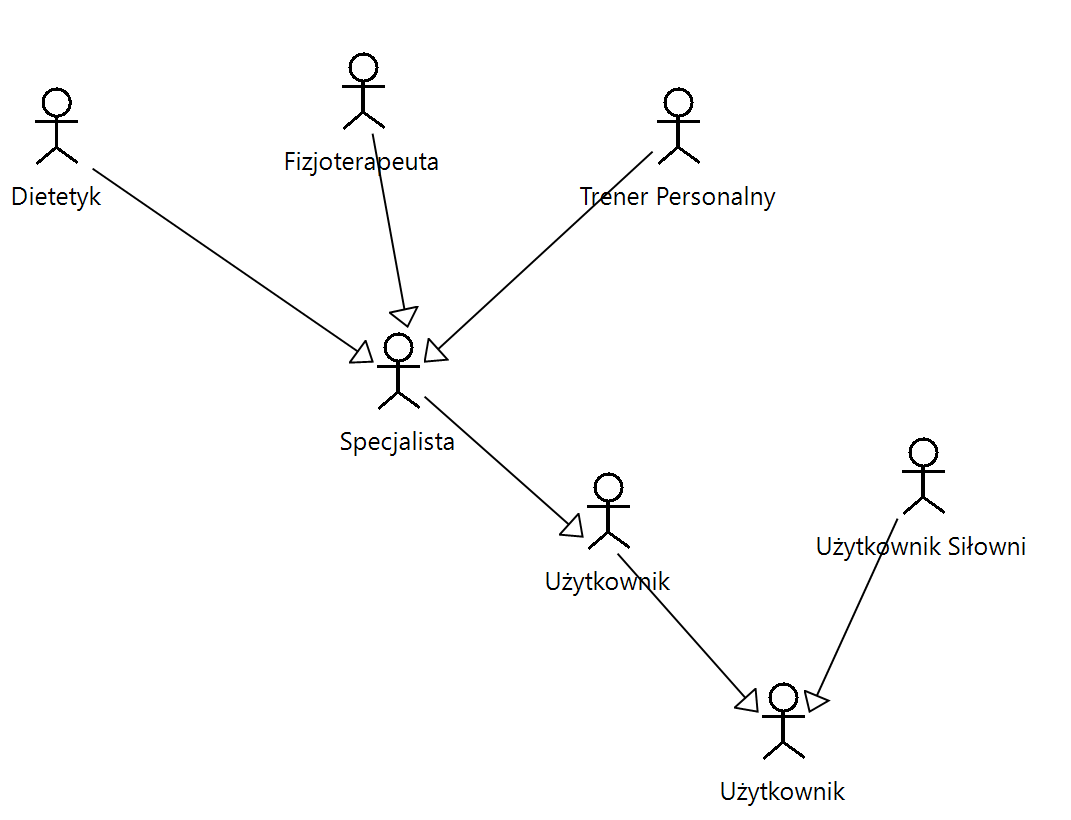
\includegraphics{diagrams/use_cases/actors_hierarchy.png}}

{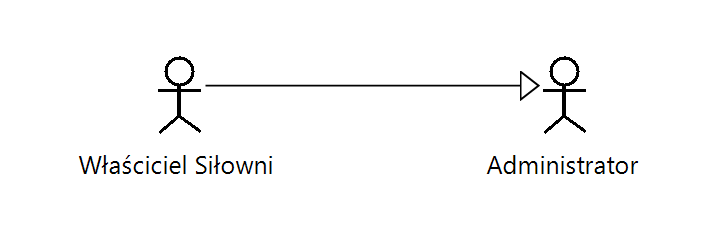
\includegraphics{diagrams/use_cases/wlasciciel_silowni_hierarchy.png}}

\hypertarget{h.9umzk2qmsz4g}{%
\subsection{\texorpdfstring{{Panel trenera
personalnego:}}{Panel trenera personalnego:}}\label{h.9umzk2qmsz4g}}

{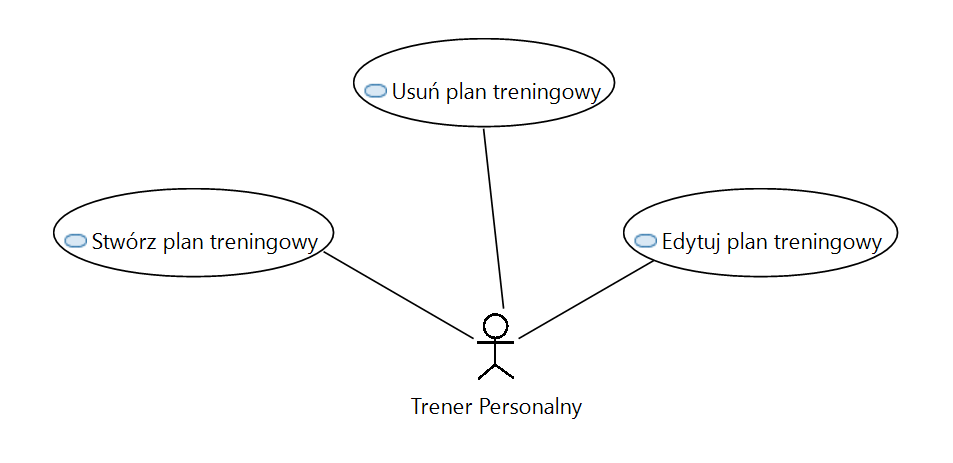
\includegraphics{diagrams/use_cases/trener_personalny.png}}
{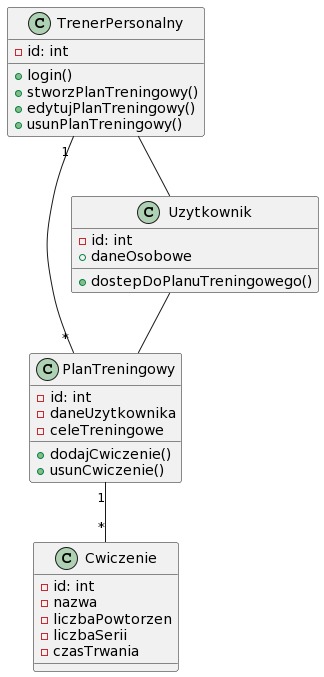
\includegraphics{diagrams/class/trener_personalny_klasy.png}}

\begin{enumerate}
\tightlist
\item
  {Stwórz plan treningowy}
\end{enumerate}

{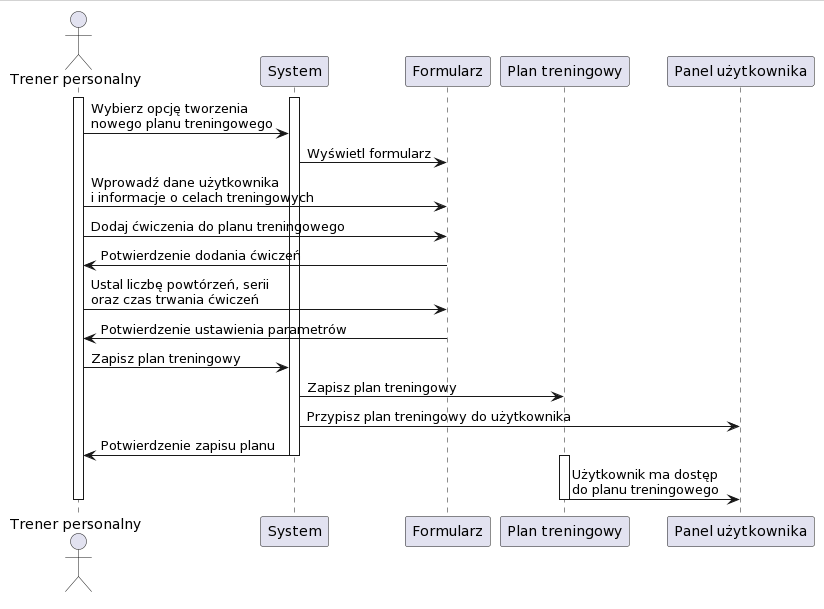
\includegraphics{diagrams/sequence/tworzenie_planu_treningu.png}}

{}

{Aktorzy biorący udział: Trener personalny}

{Cel przypadku: Stworzenie planu treningowego dla konkretnego
użytkownika.}

{Warunki początkowe: Trener personalny zalogowany w systemie, dane
użytkownika, dla którego ma być stworzony plan treningowy.}

{Warunki końcowe: Użytkownik ma dostęp do stworzonego dla niego planu
treningowego.}

{Główny ciąg zdarzeń:}

\begin{enumerate}
\tightlist
\item
  {Trener personalny wybiera opcję tworzenia nowego planu treningowego.}
\item
  {System wyświetla formularz, w którym trener personalny może
  wprowadzić dane użytkownika oraz informacje o jego celach
  treningowych.}
\item
  {Trener personalny dodaje ćwiczenia do planu treningowego, wybierając
  je z dostępnej listy lub wprowadzając nowe ćwiczenia.}
\item
  {Trener personalny ustala liczbę powtórzeń, serii oraz czas trwania
  ćwiczeń w ramach planu treningowego.}
\item
  {System zapisuje plan treningowy i przypisuje go do konta
  użytkownika.}
\item
  {Użytkownik ma dostęp do stworzonego planu treningowego w swoim panelu
  użytkownika.}
\end{enumerate}

{Alternatywne ciągi zdarzeń:}

\begin{itemize}
\tightlist
\item
  {W przypadku niekompletnych lub niepoprawnych danych trener personalny
  otrzymuje komunikat o błędzie i musi poprawić dane, aby kontynuować
  tworzenie planu treningowego.}
\item
  {Trener personalny może dodać uwagi lub informacje dodatkowe do planu
  treningowego, aby lepiej dostosować go do potrzeb użytkownika.}
\item
  {Trener personalny może edytować istniejący plan treningowy,
  zmieniając ćwiczenia, ilość serii i powtórzeń lub czas trwania
  ćwiczeń.}
\end{itemize}

{}

\begin{enumerate}
\setcounter{enumi}{1}
\tightlist
\item
  {Edytuj plan treningowy}
\end{enumerate}

{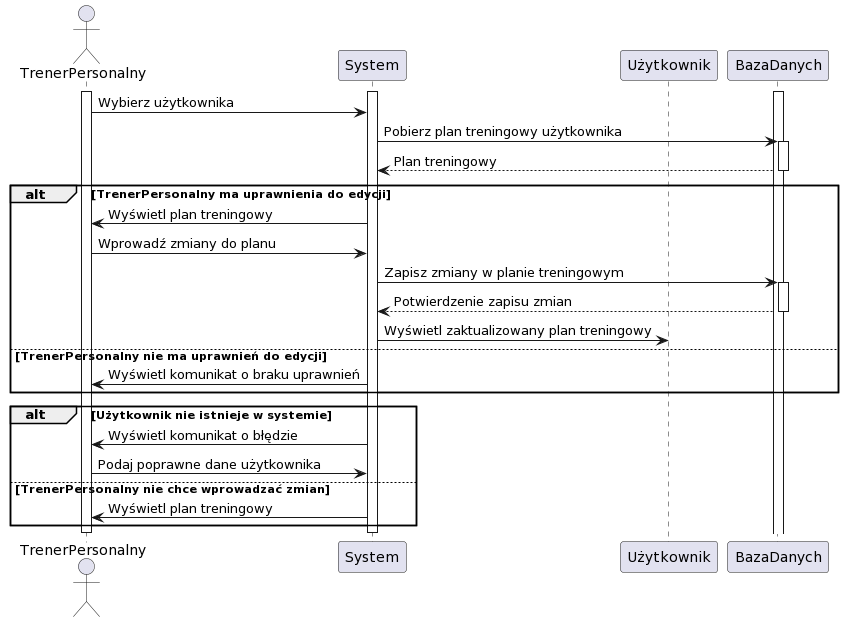
\includegraphics{diagrams/sequence/edycja_planu_treningowego.png}}

{Aktorzy biorący udział: Trener personalny}

{Cel przypadku: Umożliwienie trenerowi personalnemu wprowadzenia zmian
do istniejącego planu treningowego dla danego użytkownika.}

{Warunki początkowe: Trener personalny jest zalogowany do systemu i
posiada uprawnienia do edycji planu treningowego.}

{Warunki końcowe: Zmieniony plan treningowy jest zapisany w systemie i
jest widoczny dla użytkownika.}

{Główny ciąg zdarzeń:}

\begin{enumerate}
\tightlist
\item
  {Trener personalny wybiera użytkownika, którego plan treningowy chce
  edytować.}
\item
  {System wyświetla aktualny plan treningowy dla wybranego użytkownika.}
\item
  {Trener personalny wprowadza zmiany do planu treningowego.}
\item
  {System zapisuje zmiany i aktualizuje plan treningowy dla wybranego
  użytkownika.}
\item
  {System wyświetla potwierdzenie zapisania zmian.}
\end{enumerate}

{Alternatywne ciągi zdarzeń:}

{1a. Trener personalny nie posiada uprawnień do edycji planu
treningowego.}

\begin{itemize}
\tightlist
\item
  {System wyświetla komunikat o braku uprawnień.}
\end{itemize}

{2a. Użytkownik nie istnieje w systemie.}

\begin{itemize}
\tightlist
\item
  {System wyświetla komunikat o błędzie i prosi o podanie poprawnych
  danych.}
\end{itemize}

{3a. Trener personalny nie chce wprowadzać zmian do planu treningowego.}

\begin{itemize}
\tightlist
\item
  {System wyświetla aktualny plan treningowy dla wybranego użytkownika
  bez zmian.}
\end{itemize}

{}

\begin{enumerate}
\setcounter{enumi}{2}
\tightlist
\item
  {Usuń plan treningowy}
\end{enumerate}

{\includegraphics{diagrams/sequence/usun_plan_treningowy.png}}
{Aktorzy biorący udział: Trener personalny}

{Cel przypadku: Umożliwienie trenerowi personalnemu usunięcia planu
treningowego dla danego użytkownika.}

{Warunki początkowe: Trener personalny jest zalogowany do systemu i
posiada uprawnienia do usuwania planu treningowego.}

{Warunki końcowe: Plan treningowy dla danego użytkownika jest usunięty z
systemu.}

{Główny ciąg zdarzeń:}

\begin{enumerate}
\tightlist
\item
  {Trener personalny wybiera użytkownika, którego plan treningowy chce
  usunąć.}
\item
  {System wyświetla aktualny plan treningowy dla wybranego użytkownika.}
\item
  {Trener personalny potwierdza chęć usunięcia planu treningowego.}
\item
  {System usuwa plan treningowy z systemu.}
\item
  {System wyświetla potwierdzenie usunięcia planu treningowego.}
\end{enumerate}

{Alternatywne ciągi zdarzeń:}

{1a. Trener personalny nie posiada uprawnień do usuwania planu
treningowego.}

\begin{itemize}
\tightlist
\item
  {System wyświetla komunikat o braku uprawnień.}
\end{itemize}

{2a. Użytkownik nie istnieje w systemie.}

\begin{itemize}
\tightlist
\item
  {System wyświetla komunikat o błędzie i prosi o podanie poprawnych
  danych.}
\end{itemize}

{3a. Trener personalny nie chce usunąć planu trening}

{}

\hypertarget{h.tqqay39z8oku}{%
\subsection{\texorpdfstring{{}}{}}\label{h.tqqay39z8oku}}

{}

\hypertarget{h.vpvz4pfg93q6}{%
\subsection{\texorpdfstring{{}}{}}\label{h.vpvz4pfg93q6}}

{}

{}

{}

{}

{}

{}

{}

{}

{}

{}

\hypertarget{h.hgrtio46fsci}{%
\subsection{\texorpdfstring{{Panel
fizjoterapeuty:}}{Panel fizjoterapeuty:}}\label{h.hgrtio46fsci}}

{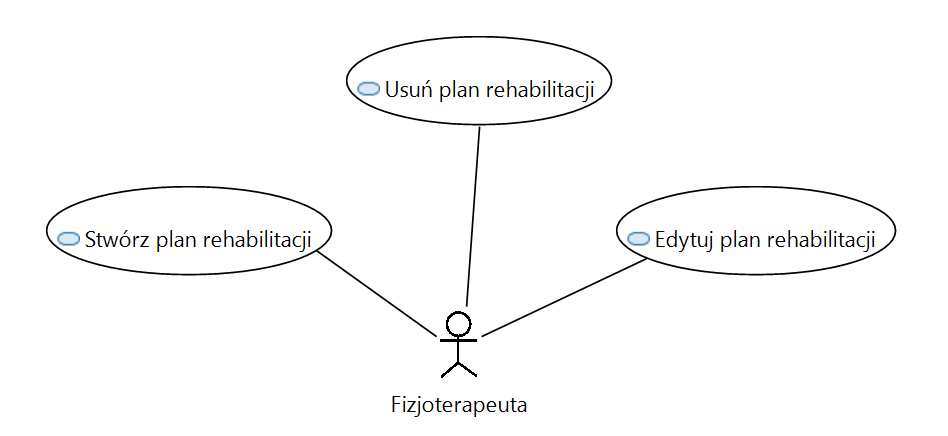
\includegraphics{diagrams/use_cases/fizjoterapeuta.png}}

\begin{enumerate}
\setcounter{enumi}{3}
\tightlist
\item
  {Stwórz plan rehabilitacji}
\end{enumerate}

{~~~~~~~~}{Aktorzy biorący udział: Fizjoterapeuta}

{~~~~~~~~Cel przypadku: Utworzenie planu rehabilitacji dla klienta}

{~~~~~~~~Warunki początkowe: Użytkownik jest zalogowany w systemie i ma
dostęp do panelu fizjoterapeuty.}

{~~~~~~~~Warunki końcowe: Utworzony został nowy plan rehabilitacji
dostępny dla klienta.}

{~~~~~~~~Główny ciąg zdarzeń:}

\begin{enumerate}
\tightlist
\item
  {Użytkownik wybiera klienta docelowego.}
\item
  {Fizjoterapeuta ~przegląda dane klienta dotyczące jego aktualnej
  diety, stylu życia oraz jego aktualnego planu treningowego.}
\item
  {Użytkownik tworzy nowy plan rehabilitacji dodając odpowiednie
  ćwiczenia oraz terminy na masaże/konsultacje.}
\item
  {Fizjoterapeuta zapisuje plan w systemie.}
\end{enumerate}

{~~~~~~~~Alternatywny ciąg zdarzeń:}

{~~~~~~~~1a. Użytkownik nie posiada uprawnień fizjoterapeuty.}

\begin{itemize}
\tightlist
\item
  {System wyświetla komunikat o braku uprawnień.}
\end{itemize}

{~~~~~~~~1b. Użytkownik nie istnieje w systemie.}

\begin{itemize}
\tightlist
\item
  {System wyświetla komunikat o błędzie i prosi o podanie poprawnych
  danych.}
\end{itemize}

{~~~~~~~~2a. Fizjoterapeuta przegląda aktualny plan rehabilitacji.}

{~~~~~~~~3a. Fizjoterapeuta dodaje nowy plan rehabilitacji, dodaje
komentarze, uwagi.}

{}

\begin{enumerate}
\setcounter{enumi}{4}
\tightlist
\item
  {Edytuj plan rehabilitacji}
\end{enumerate}

{~~~~~~~~}{Aktorzy biorący udział: Fizjoterapeuta}

{~~~~~~~~Cel przypadku: Modyfikacja istniejącego już planu
rehabilitacji}

{~~~~~~~~Warunki początkowe: Użytkownik jest zalogowany w systemie i ma
dostęp do panelu fizjoterapeuty.}

{Warunki końcowe: Zmodyfikowany został plan rehabilitacji danego
klienta}

{Główny ciąg zdarzeń:}

\begin{enumerate}
\tightlist
\item
  {Użytkownik wybiera klienta docelowego.}
\item
  {Fizjoterapeuta przegląda dane klienta, jego plan rehabilitacji.}
\item
  {Użytkownik modyfikuje plan rehabilitacji, dodając komentarze, nowe
  ćwiczenia, modyfikując lub usuwając stare.}
\item
  {Fizjoterapeuta zapisuje plan w systemie}
\end{enumerate}

{~~~~~~~~Alternatywny ciąg zdarzeń:}

{1a. Użytkownik nie posiada uprawnień fizjoterapeuty.}

\begin{itemize}
\tightlist
\item
  {System wyświetla komunikat o braku uprawnień.}
\end{itemize}

{~~~~~~~~1b. Użytkownik nie istnieje w systemie.}

\begin{itemize}
\tightlist
\item
  {System wyświetla komunikat o błędzie i prosi o podanie poprawnych
  danych.}
\end{itemize}

{2a. Brak planu rehabilitacji:}

\begin{itemize}
\tightlist
\item
  {System informuje użytkownika o braku planu rehabilitacji, daje opcję
  przejścia do panelu tworzenia nowego planu rehabilitacji.}
\end{itemize}

{}

{}

{}

{}

\begin{enumerate}
\setcounter{enumi}{5}
\tightlist
\item
  {Usuń plan rehabilitacji}{\hfill\break
  Aktorzy biorący udział: Fizjoterapeuta}
\end{enumerate}

{~~~~~~~~Cel przypadku: Usunięcie planu rehabilitacji klienta.}

{~~~~~~~~Warunki początkowe: ~Użytkownik jest zalogowany w systemie i ma
dostęp do panelu fizjoterapeuty.}

{~~~~~~~~Warunki końcowe: Plan rehabilitacji został usunięty z profilu
użytkownika.}

{~~~~~~~~Główny ciąg zdarzeń:}

\begin{enumerate}
\tightlist
\item
  {Użytkownik wybiera klienta docelowego.}
\item
  {System wyświetla aktualny plan rehabilitacji danego użytkownika.}
\item
  {Po potwierdzeniu, system usuwa plan rehabilitacji.}
\item
  {System wyświetla potwierdzenie usunięcia planu rehabilitacji.}
\end{enumerate}

{~~~~~~~~Alternatywny ciąg zdarzeń:}

{~~~~~~~~1a. Użytkownik nie posiada uprawnień fizjoterapeuty.}

\begin{itemize}
\tightlist
\item
  {System wyświetla komunikat o braku uprawnień.}
\end{itemize}

{~~~~~~~~1b. Użytkownik nie istnieje w systemie.}

\begin{itemize}
\tightlist
\item
  {System wyświetla komunikat o błędzie i prosi o podanie poprawnych
  danych.}
\end{itemize}

{~~~~~~~~2a. Brak planu rehabilitacji:}

\begin{itemize}
\tightlist
\item
  {System informuje użytkownika o braku planu rehabilitacji}
\end{itemize}

{~~~~~~~~3a. Fizjoterapeuta nie potwierdza usunięcia planu
rehabilitacji, skutkuje to informacją systemu.}

\hypertarget{h.t2karqe3ncvt}{%
\subsection{\texorpdfstring{{~~~~~~~~}}{~~~~~~~~}}\label{h.t2karqe3ncvt}}

\hypertarget{h.ks35fdzbeyq3}{%
\subsection{\texorpdfstring{{Panel
dietetyka:}}{Panel dietetyka:}}\label{h.ks35fdzbeyq3}}

{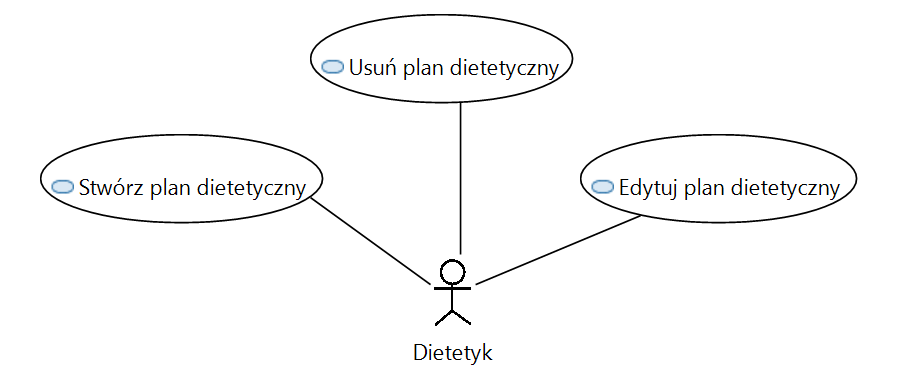
\includegraphics{diagrams/use_cases/dietetyk.png}}
{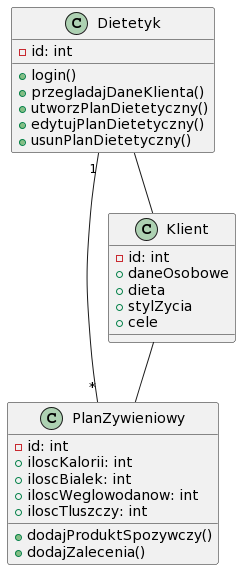
\includegraphics{diagrams/class/dietetyk.png}}

\begin{enumerate}
\setcounter{enumi}{6}
\tightlist
\item
  {Stwórz plan dietetyczny}
\end{enumerate}

{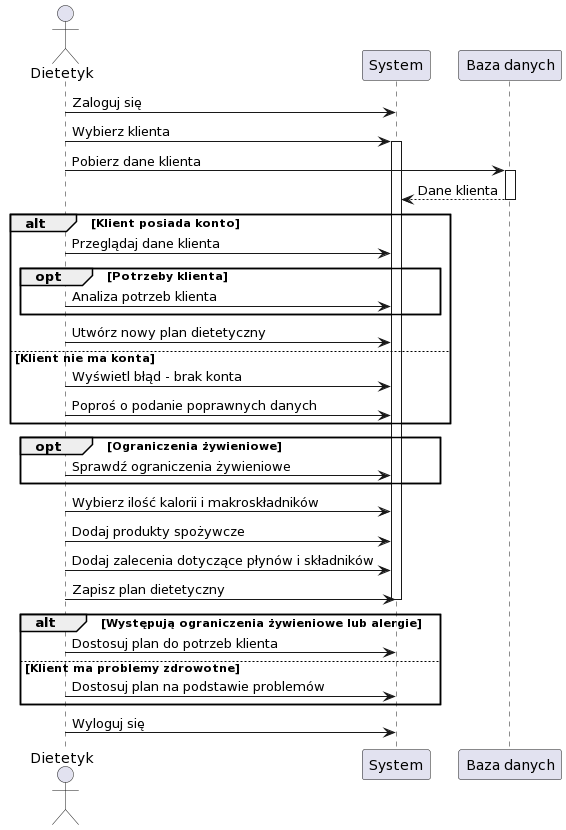
\includegraphics{diagrams/sequence/dietetyk_stworz_plan.png}}

{Aktorzy biorący udział: Dietetyk}

{Cel przypadku: Utworzenie planu dietetycznego dla klienta}

{Warunki początkowe: Dietetyk jest zalogowany do systemu i ma dostęp do
panelu dietetyka. Klient posiada konto w systemie.}

{Warunki końcowe: Utworzony jest nowy plan dietetyczny dla klienta.}

{Główny ciąg zdarzeń:}

\begin{enumerate}
\tightlist
\item
  {Dietetyk wybiera klienta, dla którego chce utworzyć plan
  dietetyczny.}
\item
  {Dietetyk przegląda dane klienta dotyczące jego aktualnej diety, stylu
  życia, celów odchudzania lub przyrostu masy mięśniowej.}
\item
  {Dietetyk tworzy nowy plan dietetyczny, wybierając odpowiednią ilość
  kalorii oraz makroskładników (białka, węglowodany, tłuszcze) dla
  klienta.}
\item
  {Dietetyk dodaje odpowiednie produkty spożywcze do planu
  dietetycznego.}
\item
  {Dietetyk dodaje zalecenia dotyczące spożycia płynów, witamin i
  minerałów.}
\item
  {Dietetyk zapisuje plan dietetyczny w systemie.}
\end{enumerate}

{Alternatywne ciągi zdarzeń:}

{2a. Jeśli klient nie ma jeszcze konta w systemie, system wyświetla błąd
i prosi o podanie poprawnych danych}

{4a. Jeśli w planie dietetycznym występują ograniczenia żywieniowe lub
alergie, dietetyk dostosowuje plan do potrzeb klienta.}

{5a. Jeśli klient ma problemy zdrowotne, dietetyk konsultuje się z
lekarzem lub innym specjalistą w celu dostosowania planu dietetycznego.}

{}

\begin{enumerate}
\setcounter{enumi}{7}
\tightlist
\item
  {Edytuj plan dietetyczny}
\end{enumerate}

{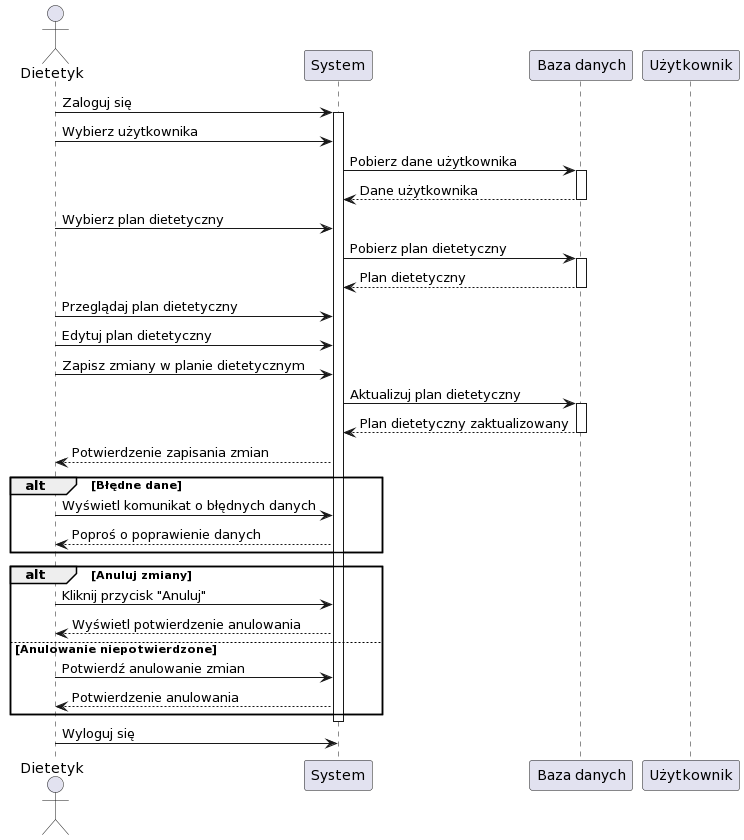
\includegraphics{diagrams/sequence/dietetyk_edytuj_plan.png}}

{Aktorzy biorący udział: Dietetyk}

{Cel przypadku: Edycja planu dietetycznego dla danego użytkownika}

{Warunki początkowe: Dietetyk zalogowany w systemie, wybrany użytkownik
oraz plan dietetyczny}

{Warunki końcowe: Plan dietetyczny dla użytkownika został
zaktualizowany}

{Główny ciąg zdarzeń:}

\begin{enumerate}
\tightlist
\item
  {Dietetyk wybiera użytkownika, dla którego chce edytować plan
  dietetyczny.}
\item
  {Dietetyk wybiera plan dietetyczny, który chce edytować.}
\item
  {System wyświetla istniejący plan dietetyczny dla użytkownika.}
\item
  {Dietetyk wprowadza zmiany w planie dietetycznym (np. zmiana posiłków,
  ilości kalorii).}
\item
  {Dietetyk zapisuje zmiany w planie dietetycznym.}
\item
  {System aktualizuje plan dietetyczny dla wybranego użytkownika.}
\item
  {System wyświetla potwierdzenie zapisania zmian w planie
  dietetycznym.}
\end{enumerate}

{Alternatywne ciągi zdarzeń:}

\begin{itemize}
\tightlist
\item
  {W przypadku błędnie wprowadzonych danych, system wyświetla odpowiedni
  komunikat i prosi o poprawienie wprowadzonych informacji.}
\item
  {Dietetyk może anulować wprowadzone zmiany, klikając przycisk
  "Anuluj". System wyświetla potwierdzenie anulowania zmian lub prosi o
  potwierdzenie przed anulowaniem.}
\end{itemize}

{}

\begin{enumerate}
\setcounter{enumi}{8}
\tightlist
\item
  {Usuń plan dietetyczny}
\end{enumerate}

{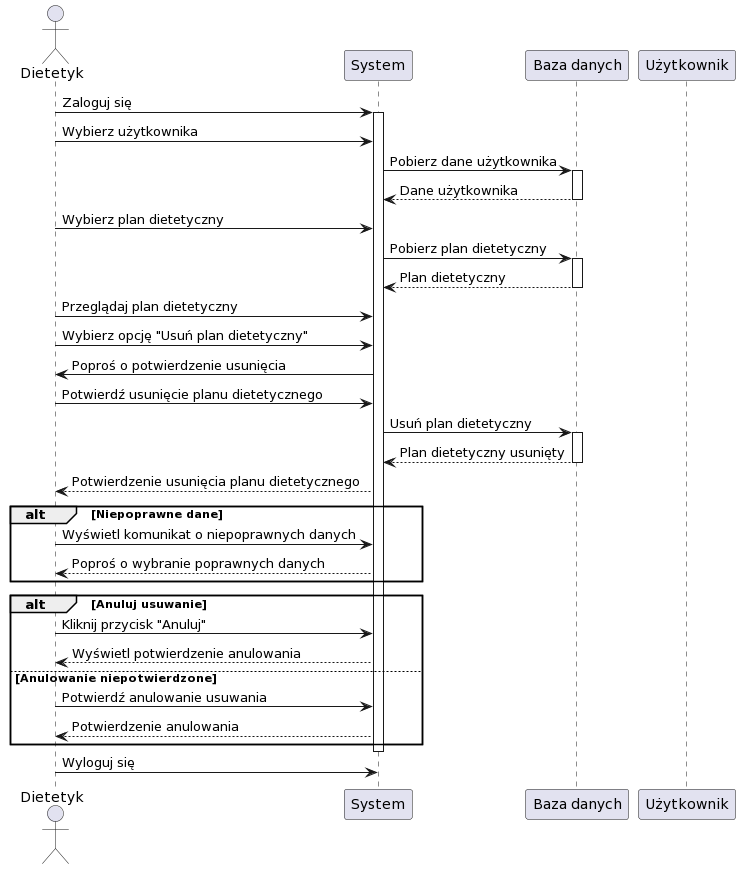
\includegraphics{diagrams/sequence/dietetyk_usun_plan.png}}
{Aktorzy biorący udział: Dietetyk}

{Cel przypadku: Usunięcie planu dietetycznego dla danego użytkownika}

{Warunki początkowe: Dietetyk zalogowany w systemie, wybrany użytkownik
oraz plan dietetyczny}

{Warunki końcowe: Plan dietetyczny dla użytkownika został usunięty}

{Główny ciąg zdarzeń:}

\begin{enumerate}
\tightlist
\item
  {Dietetyk wybiera użytkownika, dla którego chce usunąć plan
  dietetyczny.}
\item
  {Dietetyk wybiera plan dietetyczny, który chce usunąć.}
\item
  {System wyświetla istniejący plan dietetyczny dla użytkownika.}
\item
  {Dietetyk wybiera opcję "Usuń plan dietetyczny".}
\item
  {System prosi o potwierdzenie usunięcia planu dietetycznego.}
\item
  {Dietetyk potwierdza usunięcie planu dietetycznego.}
\item
  {System usuwa plan dietetyczny dla wybranego użytkownika.}
\item
  {System wyświetla potwierdzenie usunięcia planu dietetycznego.}
\end{enumerate}

{Alternatywne ciągi zdarzeń:}

\begin{itemize}
\tightlist
\item
  {W przypadku niepoprawnie wybranego użytkownika lub planu
  dietetycznego, system wyświetla odpowiedni komunikat i prosi o
  wybranie poprawnych danych.}
\item
  {Dietetyk może anulować usuwanie planu dietetycznego, klikając
  przycisk "Anuluj". System wyświetla}
\end{itemize}

\hypertarget{h.moo0g2hu8rf}{%
\subsection{\texorpdfstring{{}}{}}\label{h.moo0g2hu8rf}}

\hypertarget{h.8of6ai7v3sbh}{%
\subsection{\texorpdfstring{{Panel
specjalisty:}}{Panel specjalisty:}}\label{h.8of6ai7v3sbh}}

{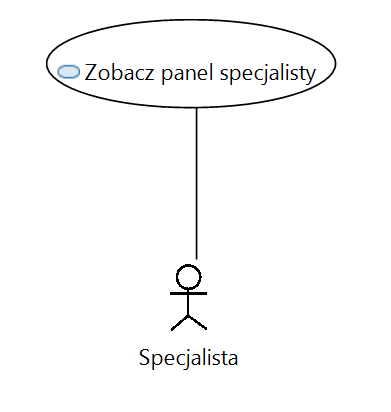
\includegraphics{diagrams/use_cases/zobacz_panel_specjalisty.png}}

\begin{enumerate}
\setcounter{enumi}{9}
\tightlist
\item
  {Zobacz panel specjalisty}
\end{enumerate}

{Aktorzy biorący udział: Specjalista (trener personalny, dietetyk,
fizjoterapeuta)}

{Cel przypadku: Wyświetlenie informacji dotyczących klientów specjalisty
i ich historii}

{Warunki początkowe: Specjalista jest zalogowany do systemu}

{Warunki końcowe: Specjalista widzi informacje dotyczące swoich klientów
i ich historii}

{Główny ciąg zdarzeń:}

\begin{enumerate}
\tightlist
\item
  {Specjalista loguje się do systemu.}
\item
  {Specjalista wybiera opcję "Panel specjalisty".}
\item
  {System wyświetla listę klientów przypisanych do specjalisty.}
\item
  {Specjalista wybiera jednego z klientów.}
\item
  {System wyświetla informacje dotyczące wybranego klienta, takie jak
  dane osobowe, historię treningów, dieta, rehabilitacja itp.}
\item
  {Specjalista może dodać notatki dotyczące wizyt i treningów klienta.}
\item
  {Specjalista kończy przeglądanie informacji i wylogowuje się z
  systemu.}
\end{enumerate}

{Alternatywne ciągi zdarzeń:}

\begin{itemize}
\tightlist
\item
  {W przypadku braku klientów przypisanych do specjalisty, system
  wyświetli stosowną informację.}
\end{itemize}

{}

\hypertarget{h.2ol8m2kl4itm}{%
\subsection{\texorpdfstring{{Panel właściciela
siłowni:}}{Panel właściciela siłowni:}}\label{h.2ol8m2kl4itm}}

{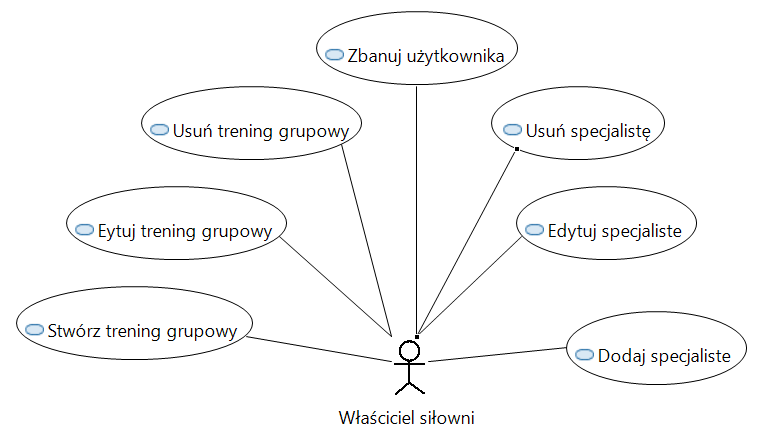
\includegraphics{diagrams/use_cases/wlasciciel_silowni.png}}

{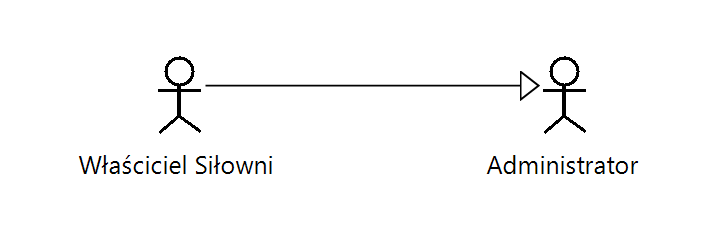
\includegraphics{diagrams/use_cases/wlasciciel_silowni_hierarchy.png}}

\begin{enumerate}
\setcounter{enumi}{10}
\tightlist
\item
  {Stwórz trening grupowy}
\end{enumerate}

{~~~~~~~~}{Aktorzy biorący udział: Właściciel siłowni}

{~~~~~~~~Cel przypadku: Utworzenie treningu grupowego dla klientów.}

{~~~~~~~~Warunki początkowe: Właściciel siłowni jest zalogowany w
systemie i ma dostęp do panelu właściciela siłowni.}

{~~~~~~~~Warunki końcowe: Utworzony trening grupowy, który jest dostępny
dla użytkowników.}

{~~~~~~~~Główny ciąg zdarzeń:}

\begin{enumerate}
\tightlist
\item
  {Właściciel siłowni wybiera opcję "Tworzenie treningu grupowego".}
\item
  {System wyświetla formularz, w którym właściciel siłowni może
  wprowadzić informacje dotyczące treningu, takie jak:}
\end{enumerate}

\begin{itemize}
\tightlist
\item
  {Nazwa treningu}
\item
  {Data i godzina rozpoczęcia}
\item
  {Czas trwania treningu}
\item
  {Maksymalna liczba uczestników}
\item
  {Opis treningu (np. rodzaj ćwiczeń, poziom trudności itp.)}
\end{itemize}

\begin{enumerate}
\setcounter{enumi}{2}
\tightlist
\item
  {Użytkownik uzupełnia formularz i zapisuje trening.}
\item
  {System potwierdza utworzenie treningu i automatycznie dodaje go do
  harmonogramu zajęć w aplikacji siłowni.}
\end{enumerate}

{~~~~~~~~Alternatywne ciąg zdarzeń:}

\begin{itemize}
\tightlist
\item
  {Użytkownik nie posiada uprawnień właściciela siłowni.}
\end{itemize}

\begin{itemize}
\tightlist
\item
  {System wyświetla komunikat o braku uprawnień.}
\end{itemize}

\begin{itemize}
\tightlist
\item
  {Użytkownik wprowadził niepoprawne dane w formularzu.}
\end{itemize}

\begin{itemize}
\tightlist
\item
  {System wyświetla komunikat o niepoprawnie wprowadzonych danych i
  prosi o poprawienie danych.}
\end{itemize}

{}

\begin{enumerate}
\setcounter{enumi}{11}
\tightlist
\item
  {Edytuj trening grupowy}
\end{enumerate}

{Aktorzy biorący udział: Właściciel siłowni}

{~~~~~~~~Cel przypadku: Edycja treningu grupowego.}

{~~~~~~~~Warunki początkowe: Właściciel siłowni jest zalogowany w
systemie i ma dostęp do panelu właściciela siłowni.}

{~~~~~~~~Warunki końcowe: Zaktualizowany trening grupowy.}

{~~~~~~~~Główny ciąg zdarzeń:}

\begin{enumerate}
\tightlist
\item
  {Właściciel siłowni otwiera okno treningów grupowych.}
\item
  {Użytkownik wybiera odpowiedni trening grupowy.}
\item
  {System wyświetla dane treningu z możliwością edycji każdego pola.}
\item
  {Właściciel siłowni }{edytuje}{~i zapisuje dane.}
\item
  {~System potwierdza wprowadzone zmiany}
\end{enumerate}

{~~~~~~~~Alternatywny ciąg zdarzeń:}

\begin{itemize}
\tightlist
\item
  {Użytkownik nie posiada uprawnień właściciela siłowni.}
\end{itemize}

\begin{itemize}
\tightlist
\item
  {System wyświetla komunikat o braku uprawnień.}
\end{itemize}

\begin{itemize}
\tightlist
\item
  {Użytkownik wprowadził niepoprawne dane w formularzu.}
\end{itemize}

\begin{itemize}
\tightlist
\item
  {System wyświetla komunikat o niepoprawnie wprowadzonych danych i
  prosi o poprawienie danych.}
\end{itemize}

\begin{itemize}
\tightlist
\item
  {Użytkownik nie wprowadził zmian.}
\end{itemize}

{\hfill\break
}

\begin{enumerate}
\setcounter{enumi}{12}
\tightlist
\item
  {Usuń trening grupowy}
\end{enumerate}

{Aktorzy biorący udział: Właściciel siłowni}

{~~~~~~~~Cel przypadku: Usunięcie w systemie treningu grupowego.}

{~~~~~~~~Warunki początkowe: Właściciel siłowni jest zalogowany w
systemie i ma dostęp do panelu właściciela siłowni.}

{~~~~~~~~Warunki końcowe: Trening grupowy został usunięty.}

{~~~~~~~~Główny ciąg zdarzeń:}

\begin{enumerate}
\tightlist
\item
  {Właściciel siłowni otwiera okno treningów grupowych.}
\item
  {Użytkownik wybiera odpowiedni trening.}
\item
  {Właściciel siłowni wybiera opcję ``Usuń'' i potwierdza.}
\item
  {System potwierdza usunięcie treningu grupowego.}
\end{enumerate}

{~~~~~~~~Alternatywny ciąg zdarzeń:}

\begin{itemize}
\tightlist
\item
  {Użytkownik nie posiada uprawnień właściciela siłowni.}
\end{itemize}

\begin{itemize}
\tightlist
\item
  {System wyświetla komunikat o braku uprawnień.}
\end{itemize}

\begin{itemize}
\tightlist
\item
  {Brak treningów grupowych.}
\end{itemize}

\begin{itemize}
\tightlist
\item
  {System wyświetla komunikat o braku treningów grupowych.}
\end{itemize}

\begin{itemize}
\tightlist
\item
  {Właściciel siłowni nie potwierdził usunięcia.\\
  }
\end{itemize}

\begin{enumerate}
\setcounter{enumi}{13}
\tightlist
\item
  {Zbanuj użytkownika}
\end{enumerate}

{Aktorzy biorący udział: Właściciel siłowni}

{~~~~~~~~Cel przypadku: Zbanowanie użytkownika.}

{~~~~~~~~Warunki początkowe: Właściciel siłowni jest zalogowany w
systemie i ma dostęp do panelu właściciela siłowni.}

{~~~~~~~~Warunki końcowe: Wybrany użytkownik został zbanowany w
systemie.}

{~~~~~~~~Główny ciąg zdarzeń:}

\begin{enumerate}
\tightlist
\item
  {Właściciel siłowni otwiera listę użytkowników swojej siłowni.}
\item
  {Użytkownik wybiera osobę którą chce zbanować i potwierdza.}
\item
  {System zwraca komunikat potwierdzający zbanowanie użytkownika.}
\end{enumerate}

{~~~~~~~~Alternatywny ciąg zdarzeń:}

\begin{itemize}
\tightlist
\item
  {Użytkownik nie posiada uprawnień właściciela siłowni.}
\end{itemize}

\begin{itemize}
\tightlist
\item
  {System wyświetla komunikat o braku uprawnień.}
\end{itemize}

\begin{itemize}
\tightlist
\item
  {Brak użytkowników siłowni.}
\end{itemize}

\begin{itemize}
\tightlist
\item
  {System wyświetla komunikat o braku użytkowników.}
\end{itemize}

\begin{itemize}
\tightlist
\item
  {Właściciel siłowni nie potwierdził zbanowania.\\
  }
\end{itemize}

{}

{}

{}

{}

{}

{}

{}

\begin{enumerate}
\setcounter{enumi}{14}
\tightlist
\item
  {Dodaj specjalistę}
\end{enumerate}

{Aktorzy biorący udział: Właściciel siłowni}

{~~~~~~~~Cel przypadku: Dodanie w systemie specjalisty}

{~~~~~~~~Warunki początkowe: Właściciel siłowni jest zalogowany w
systemie i ma dostęp do panelu właściciela siłowni.}

{~~~~~~~~Warunki końcowe: Specjalista został dodany w systemie i jest
dostępny dla użytkowników.}

{~~~~~~~~Główny ciąg zdarzeń:}

\begin{enumerate}
\tightlist
\item
  {Właściciel siłowni otwiera okno ``Specjaliści''.}
\item
  {Użytkownik wybiera opcję ``Dodaj Specjalistę''.}
\item
  {System wyświetla formularz, w którym właściciel siłowni może
  wprowadzić informacje dotyczące specjalisty, takie jak:}
\end{enumerate}

\begin{itemize}
\tightlist
\item
  {Imię, Nazwisko}
\item
  {Numer telefonu}
\item
  {Rodzaj specjalisty}
\item
  {Godziny pracy}
\end{itemize}

\begin{enumerate}
\setcounter{enumi}{3}
\tightlist
\item
  {Użytkownik uzupełnia formularz i zapisuje w systemie.}
\item
  {System potwierdza dodanie specjalisty i dodaje go do listy dostępnych
  specjalistów dla użytkowników siłowni.}
\end{enumerate}

{~~~~~~~~Alternatywny ciąg zdarzeń:}

\begin{itemize}
\tightlist
\item
  {Użytkownik nie posiada uprawnień właściciela siłowni.}
\end{itemize}

\begin{itemize}
\tightlist
\item
  {System wyświetla komunikat o braku uprawnień.}
\end{itemize}

\begin{itemize}
\tightlist
\item
  {Właściciel siłowni otwiera listę użytkowników swojej siłowni.}
\end{itemize}

\begin{itemize}
\tightlist
\item
  {Wybiera odpowiedniego użytkownika i wybiera opcję ``Ustaw jako
  specjalistę''.}
\item
  {System wysyła zapytanie do użytkownika wraz z formularzem.}
\item
  {System potwierdza dodanie specjalisty i dodaje go do listy dostępnych
  specjalistów dla użytkowników siłowni.}
\end{itemize}

\begin{itemize}
\tightlist
\item
  {Użytkownik nie potwierdza zapytania/ nie wypełnia formularza.}
\item
  {Użytkownik/ Właściciel siłowni wprowadził niepoprawne dane w
  formularzu.}
\end{itemize}

\begin{itemize}
\tightlist
\item
  {System wyświetla komunikat o niepoprawnie wprowadzonych danych i
  prosi o poprawienie danych.\\
  }
\end{itemize}

\begin{enumerate}
\setcounter{enumi}{15}
\tightlist
\item
  {Edytuj specjalistę}
\end{enumerate}

{Aktorzy biorący udział: Właściciel siłowni}

{~~~~~~~~Cel przypadku: Edycja danych specjalisty.}

{~~~~~~~~Warunki początkowe: Właściciel siłowni jest zalogowany w
systemie i ma dostęp do panelu właściciela siłowni.}

{~~~~~~~~Warunki końcowe: Modyfikacja danych specjalisty.}

{~~~~~~~~Główny ciąg zdarzeń:}

\begin{enumerate}
\tightlist
\item
  {Właściciel siłowni otwiera okno ``Specjaliści''.}
\item
  {Użytkownik wybiera specjalistę docelowego.}
\item
  {Właściciel siłowni wybiera opcję ``Edytuj''.}
\item
  {Po edycji i danych i potwierdzeniu czynności system potwierdza
  zapisaną akcję.}
\item
  {Specjalista, którego były modyfikowane dane potwierdza wprowadzone
  zmiany.}
\item
  {Dane są zapisane w systemie i dostępne dla użytkowników.}
\end{enumerate}

{~~~~~~~~Alternatywny ciąg zdarzeń:}

\begin{itemize}
\tightlist
\item
  {Użytkownik nie posiada uprawnień właściciela siłowni.}
\end{itemize}

\begin{itemize}
\tightlist
\item
  {System wyświetla komunikat o braku uprawnień.}
\end{itemize}

\begin{itemize}
\tightlist
\item
  {Użytkownik wprowadził niepoprawne dane w formularzu.}
\end{itemize}

\begin{itemize}
\tightlist
\item
  {System wyświetla komunikat o niepoprawnie wprowadzonych danych i
  prosi o poprawienie danych.}
\end{itemize}

\begin{itemize}
\tightlist
\item
  {Użytkownik nie wprowadził zmian.}
\item
  {Dany specjalista nie potwierdził zmian}
\end{itemize}

{\hfill\break
}

\begin{enumerate}
\setcounter{enumi}{16}
\tightlist
\item
  {Usuń specjalistę}
\end{enumerate}

{Aktorzy biorący udział: Właściciel siłowni}

{~~~~~~~~Cel przypadku: Usunięcie użytkownika z listy specjalistów.}

{~~~~~~~~Warunki początkowe: Właściciel siłowni jest zalogowany w
systemie i ma dostęp do panelu właściciela siłowni.}

{~~~~~~~~Warunki końcowe: Usunięty specjalista.}

{~~~~~~~~Główny ciąg zdarzeń:}

\begin{enumerate}
\tightlist
\item
  {Właściciel siłowni otwiera okno ``Specjaliści''.}
\item
  {Użytkownik wybiera specjalistę docelowego.}
\item
  {Właściciel siłowni wybiera opcję ``Usuń'' i potwierdza.}
\item
  {Po potwierdzeniu system zwraca informację o poprawnie usuniętym
  specjaliście.}
\end{enumerate}

{Alternatywny ciąg zdarzeń:}

\begin{itemize}
\tightlist
\item
  {~Użytkownik nie posiada uprawnień właściciela siłowni.}
\end{itemize}

\begin{itemize}
\tightlist
\item
  {System wyświetla komunikat o braku uprawnień.}
\end{itemize}

\begin{itemize}
\tightlist
\item
  {Brak specjalistów}
\end{itemize}

\begin{itemize}
\tightlist
\item
  {System wyświetla komunikat o braku specjalistów.}
\end{itemize}

\begin{itemize}
\tightlist
\item
  {Właściciel siłowni nie potwierdził usunięcia użytkownika. }
\end{itemize}

{}

{}

\begin{enumerate}
\setcounter{enumi}{17}
\tightlist
\item
  {Przypisz specjalistę do budynku}
\end{enumerate}

{Aktorzy biorący udział: Właściciel siłowni}

{~~~~~~~~Cel przypadku: Przypisanie specjalisty do danego budynku.}

{~~~~~~~~Warunki początkowe: Właściciel siłowni jest zalogowany w
systemie i ma dostęp do panelu właściciela siłowni.}

{~~~~~~~~Warunki końcowe: Specjalista przypisany do budynku.}

{~~~~~~~~Główny ciąg zdarzeń:}

\begin{enumerate}
\tightlist
\item
  {Właściciel siłowni otwiera okno ``Specjaliści''.}
\item
  {Użytkownik wybiera specjalistę docelowego.}
\item
  {Właściciel siłowni wybiera opcję ``Przypisz specjalistę do budynku''
  i wybiera z listy odpowiednią placówkę.}
\item
  {System zwraca informację o poprawnie wykonanej akcji.}
\end{enumerate}

{~~~~~~~~Alternatywny ciąg zdarzeń:}

\begin{itemize}
\tightlist
\item
  {~ Użytkownik nie posiada uprawnień właściciela siłowni.}
\end{itemize}

\begin{itemize}
\tightlist
\item
  {System wyświetla komunikat o braku uprawnień.}
\end{itemize}

\begin{itemize}
\tightlist
\item
  {Brak specjalistów}
\end{itemize}

\begin{itemize}
\tightlist
\item
  {System wyświetla komunikat o braku specjalistów.}
\end{itemize}

{}

{}

\begin{itemize}
\tightlist
\item
  {Istnieje tylko 1 placówka }
\end{itemize}

\begin{itemize}
\tightlist
\item
  {Specjalista jest automatycznie przypisywany do tej placówki.\\
  }
\end{itemize}

\begin{enumerate}
\setcounter{enumi}{18}
\tightlist
\item
  {Usuń specjalistę z budynku}
\end{enumerate}

{Aktorzy biorący udział: Właściciel siłowni}

{~~~~~~~~Cel przypadku: Usunięcie specjalisty z budynku.}

{~~~~~~~~Warunki początkowe: Właściciel siłowni jest zalogowany w
systemie i ma dostęp do panelu właściciela siłowni.}

{~~~~~~~~Warunki końcowe: Specjalista został usunięty z budynku.}

{~~~~~~~~Główny ciąg zdarzeń:}

\begin{enumerate}
\tightlist
\item
  {Właściciel siłowni otwiera okno ``Specjaliści''.}
\item
  {Użytkownik wybiera specjalistę docelowego.}
\item
  {Właściciel siłowni wybiera opcję ``Usuń specjalistę z budynku'' i
  potwierdza czynność.}
\item
  {System zwraca informację z potwierdzeniem czynności i wysyła prośbę
  do usuniętego specjalisty o dodatkowe potwierdzenie.}
\item
  {Specjalista jest usunięty z danego budynku, dane dla użytkowników są
  zaktualizowane.}
\end{enumerate}

{~~~~~~~~Alternatywny ciąg zdarzeń:}

\begin{itemize}
\tightlist
\item
  {~ Użytkownik nie posiada uprawnień właściciela siłowni.}
\end{itemize}

\begin{itemize}
\tightlist
\item
  {System wyświetla komunikat o braku uprawnień.}
\end{itemize}

\begin{itemize}
\tightlist
\item
  {Brak specjalistów}
\end{itemize}

\begin{itemize}
\tightlist
\item
  {System wyświetla komunikat o braku specjalistów.}
\end{itemize}

\begin{itemize}
\tightlist
\item
  {Właściciel siłowni nie potwierdził usunięcia specjalisty z budynku.}
\item
  {Specjalista nie potwierdził usunięcia z danego budynku.\\
  }
\end{itemize}

{}

{}

{}

\begin{enumerate}
\setcounter{enumi}{19}
\tightlist
\item
  {Wypisz użytkownika z treningu personalnego}
\end{enumerate}

{Aktorzy biorący udział: Właściciel siłowni}

{Cel przypadku: Usunięcie użytkownika z listy uczestników treningu
personalnego}

{Warunki początkowe: Właściciel siłowni ~jest zalogowany do systemu,
użytkownik jest zapisany na trening personalny}

{Warunki końcowe: Użytkownik zostaje usunięty z listy uczestników
treningu personalnego}

{Główny ciąg zdarzeń:}

\begin{enumerate}
\tightlist
\item
  {Właściciel siłowni loguje się do systemu.}
\item
  {Właściciel siłowni wybiera opcję "Zarządzanie treningami
  personalnymi".}
\item
  {System wyświetla listę zapisanych na trening personalny
  użytkowników.}
\item
  {Właściciel siłowni wybiera użytkownika, którego chce usunąć z
  treningu personalnego.}
\item
  {System wyświetla szczegóły zapisu użytkownika na trening personalny.}
\item
  {Właściciel siłowni wybiera opcję "Usuń użytkownika".}
\item
  {System usuwa użytkownika z listy uczestników treningu personalnego i
  wyświetla stosowną informację.}
\item
  {Właściciel siłowni kończy procedurę i wylogowuje się z systemu.}
\end{enumerate}

{Alternatywne ciągi zdarzeń:}

\begin{itemize}
\tightlist
\item
  {W przypadku, gdy użytkownik nie jest zapisany na trening personalny,
  system wyświetli stosowną informację.}
\item
  {W przypadku, gdy użytkownik ma już opłacony trening personalny,
  system zapyta, czy chce zwrócić pieniądze użytkownikowi lub przesunąć
  go na inny trening personalny.}
\end{itemize}

{}

{}

\begin{enumerate}
\setcounter{enumi}{20}
\tightlist
\item
  {Wypisz użytkownika z treningu grupowego}
\end{enumerate}

{Aktorzy biorący udział: Właściciel siłowni}

{Cel przypadku: Usunięcie użytkownika z rezerwacji na trening grupowy.}

{Warunki początkowe: Użytkownik jest zarejestrowany na trening grupowy,
trening grupowy jest zaplanowany na konkretny dzień i godzinę.}

{Warunki końcowe: Użytkownik został usunięty z rezerwacji na trening
grupowy.}

{Główny ciąg zdarzeń:}

\begin{enumerate}
\tightlist
\item
  {Właściciel siłowni loguje się do systemu.}
\item
  {Właściciel siłowni znajduje użytkownika na liście uczestników
  treningu grupowego.}
\item
  {Właściciel siłowni usuwa użytkownika z rezerwacji na trening
  grupowy.}
\item
  {System wyświetla komunikat potwierdzający usunięcie użytkownika.}
\end{enumerate}

{Alternatywne ciągi zdarzeń:}

\begin{itemize}
\tightlist
\item
  {Jeśli użytkownik nie został znaleziony na liście uczestników treningu
  grupowego, system wyświetla komunikat o błędzie i prosi o wprowadzenie
  poprawnych danych.}
\item
  {Jeśli trening grupowy został odwołany lub zmieniony, system wyświetla
  komunikat informujący o zmianach i proponuje przypisanie użytkownika
  do innego treningu grupowego.}
\end{itemize}

{}

{}

{}

\begin{enumerate}
\setcounter{enumi}{21}
\tightlist
\item
  {Wypisz użytkownika z rehabilitacji}
\end{enumerate}

{Aktorzy biorący udział: Właściciel siłowni}

{Cel przypadku: Usunięcie użytkownika z listy uczestników rehabilitacji}

{Warunki początkowe: Właściciel siłowni jest zalogowany do systemu i
posiada uprawnienia do zarządzania rehabilitacją}

{Warunki końcowe: Użytkownik zostaje usunięty z listy uczestników
rehabilitacji}

{Główny ciąg zdarzeń:}

\begin{enumerate}
\tightlist
\item
  {Właściciel siłowni wybiera moduł zarządzania rehabilitacją}
\item
  {Właściciel siłowni wyszukuje użytkownika, którego chce usunąć z listy
  uczestników rehabilitacji}
\item
  {Właściciel siłowni otwiera kartę użytkownika i wybiera opcję "Usuń
  użytkownika z listy rehabilitacji"}
\item
  {System wyświetla komunikat potwierdzający operację usuwania}
\item
  {Właściciel siłowni potwierdza chęć usunięcia użytkownika z listy
  uczestników rehabilitacji}
\item
  {System usuwa użytkownika z listy uczestników rehabilitacji}
\item
  {System wyświetla potwierdzenie usunięcia użytkownika z listy
  uczestników rehabilitacji}
\end{enumerate}

{Alternatywne ciągi zdarzeń:}

\begin{itemize}
\tightlist
\item
  {Jeśli użytkownik nie jest obecny na liście uczestników rehabilitacji,
  to właściciel siłowni otrzymuje komunikat informujący o tym fakcie.}
\item
  {Jeśli wystąpią problemy z usunięciem użytkownika z listy uczestników
  rehabilitacji, system wyświetli komunikat z informacją o błędzie.}
\end{itemize}

{}

{}

\begin{enumerate}
\setcounter{enumi}{22}
\tightlist
\item
  {Wypisz użytkownika z wizyty u dietetyka}
\end{enumerate}

{Aktorzy biorący udział: Właściciel siłowni}

{Cel przypadku: Usunięcie użytkownika z listy zarejestrowanych na wizytę
u dietetyka}

{Warunki początkowe: Właściciel siłowni jest zalogowany do systemu,
użytkownik jest zarejestrowany na wizytę u dietetyka}

{Warunki końcowe: Użytkownik zostaje usunięty z listy zarejestrowanych
na wizytę u dietetyka}

{Główny ciąg zdarzeń:}

\begin{enumerate}
\tightlist
\item
  {Właściciel siłowni wybiera opcję zarządzania wizytami u dietetyka.}
\item
  {System wyświetla listę użytkowników zarejestrowanych na wizytę u
  dietetyka.}
\item
  {Właściciel siłowni wybiera użytkownika, którego chce wypisać z
  wizyty.}
\item
  {System wyświetla potwierdzenie usunięcia użytkownika z listy
  zarejestrowanych na wizytę.}
\item
  {Właściciel siłowni potwierdza usunięcie użytkownika.}
\item
  {System usuwa użytkownika z listy zarejestrowanych na wizytę u
  dietetyka.}
\item
  {System wyświetla potwierdzenie usunięcia użytkownika z listy.}
\end{enumerate}

{Alternatywne ciągi zdarzeń:}

\begin{itemize}
\tightlist
\item
  {~Jeśli właściciel siłowni nie może znaleźć użytkownika na liście
  zarejestrowanych na wizytę u dietetyka, to system wyświetla komunikat
  informujący o tym fakcie.}
\end{itemize}

{}

{}

{}

\begin{enumerate}
\setcounter{enumi}{23}
\tightlist
\item
  {Wygeneruj statystyki}
\end{enumerate}

{Aktorzy biorący udział: Właściciel siłowni}

{Cel przypadku: Wygenerowanie różnych statystyk dotyczących działalności
siłowni, takich jak przychody, ilość użytkowników, popularność zajęć,
wykorzystanie sprzętu.}

{Warunki początkowe: Właściciel siłowni jest zalogowany do systemu
zarządzania siłownią.}

{Warunki końcowe: Wygenerowanie i wyświetlenie statystyk dotyczących
działalności siłowni.}

{Główny ciąg zdarzeń:}

\begin{enumerate}
\tightlist
\item
  {Właściciel siłowni wybiera moduł zarządzania finansami.}
\item
  {Właściciel siłowni wybiera opcję "Wygeneruj statystyki".}
\item
  {System wyświetla różne opcje statystyk do wyboru, takie jak
  przychody, ilość użytkowników, popularność zajęć itp.}
\item
  {Właściciel siłowni wybiera interesującą go opcję statystyk.}
\item
  {System generuje statystyki i wyświetla je na ekranie.}
\item
  {Właściciel siłowni może wydrukować lub pobrać statystyki w formacie
  pliku.}
\end{enumerate}

{Alternatywne ciągi zdarzeń:}

\begin{itemize}
\tightlist
\item
  {Jeśli system nie może wygenerować statystyk z powodu braku danych,
  wyświetlany jest komunikat informujący o tym fakcie. Właściciel
  siłowni może wtedy zdecydować się na inne statystyki lub wykonać
  czynności, które umożliwią generowanie wybranych statystyk.}
\end{itemize}

\hypertarget{h.sjnlhh288rjz}{%
\subsection{\texorpdfstring{{Panel
Administratora:}}{Panel Administratora:}}\label{h.sjnlhh288rjz}}

{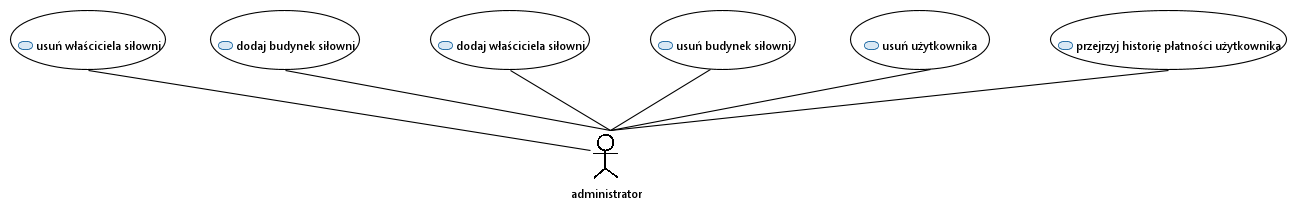
\includegraphics{diagrams/use_cases/administrator.png}}

\begin{enumerate}
\setcounter{enumi}{24}
\tightlist
\item
  {Przejrzyj historię płatności użytkownika}
\end{enumerate}

{Aktorzy biorący udział: Administrator}

{Cel przypadku: Przejrzenie historii płatności konkretnego użytkownika}

{Warunki początkowe: Administrator jest zalogowany do systemu i ma
uprawnienia do przeglądania historii płatności użytkowników.}

{Warunki końcowe: Administrator ma dostęp do szczegółowej historii
płatności użytkownika.}

{Główny ciąg zdarzeń:}

\begin{enumerate}
\tightlist
\item
  {Administrator wybiera opcję "Historia płatności" w panelu
  administratora.}
\item
  {System wyświetla listę użytkowników, którzy dokonali płatności.}
\item
  {Administrator wybiera użytkownika, którego historię płatności chce
  przeglądać.}
\item
  {System wyświetla szczegółową historię płatności wybranego
  użytkownika, w tym daty, kwoty oraz rodzaj płatności.}
\item
  {Administrator może przeglądać historię płatności użytkownika, a także
  eksportować ją do pliku CSV lub PDF.}
\item
  {Po zakończeniu przeglądania historii płatności, administrator może
  wrócić do panelu administratora lub wylogować się z systemu.}
\end{enumerate}

{Alternatywne ciągi zdarzeń:}

\begin{itemize}
\tightlist
\item
  {Jeśli nie ma żadnych użytkowników z dokonanymi płatnościami, system
  wyświetla komunikat, że nie ma historii płatności do wyświetlenia.}
\item
  {Jeśli nie można znaleźć użytkownika, administrator otrzymuje
  komunikat, że nie ma użytkownika o podanym adresie e-mail lub
  loginie.}
\end{itemize}

{}

{}

\begin{enumerate}
\setcounter{enumi}{25}
\tightlist
\item
  {Dodaj budynek siłowni}
\end{enumerate}

{Aktorzy biorący udział: Administrator}

{Cel przypadku: Dodanie nowego budynku siłowni do systemu zarządzania
siłownią}

{Warunki początkowe: Administrator zalogowany do systemu, posiadający
uprawnienia do dodawania nowych budynków siłowni}

{Warunki końcowe: Nowy budynek siłowni został dodany do systemu i jest
dostępny dla użytkowników}

{Główny ciąg zdarzeń:}

\begin{enumerate}
\tightlist
\item
  {Administrator wybiera opcję "Dodaj budynek siłowni"}
\item
  {System wyświetla formularz dodawania nowego budynku siłowni}
\item
  {Administrator wprowadza nazwę budynku, adres, numer telefonu i adres
  e-mail}
\item
  {Administrator wybiera zdjęcie budynku z dysku lub podaje adres URL}
\item
  {Administrator zatwierdza dodanie nowego budynku siłowni}
\item
  {System dodaje nowy budynek siłowni do bazy danych}
\item
  {System wyświetla komunikat potwierdzający dodanie nowego budynku
  siłowni}
\end{enumerate}

{Alternatywne ciągi zdarzeń:}

\begin{itemize}
\tightlist
\item
  {W przypadku błędnie wprowadzonych danych, system wyświetla komunikat
  o błędach i prosi o ich poprawienie.}
\item
  {Administrator może zrezygnować z dodania nowego budynku siłowni,
  klikając opcję "Anuluj". W takim przypadku system nie dodaje nowego
  budynku i zamyka formularz.}
\end{itemize}

{}

{}

\begin{enumerate}
\setcounter{enumi}{26}
\tightlist
\item
  {Dodaj właściciela siłowni}
\end{enumerate}

{Aktorzy biorący udział: Administrator}

{Cel przypadku: Dodanie nowego właściciela siłowni do systemu}

{Warunki początkowe: Administrator zalogowany do systemu}

{Warunki końcowe: Nowy właściciel siłowni dodany do systemu}

{Główny ciąg zdarzeń:}

\begin{enumerate}
\tightlist
\item
  {Administrator wybiera opcję "Dodaj właściciela siłowni" z panelu
  administracyjnego.}
\item
  {System wyświetla formularz dodawania nowego właściciela siłowni z
  polami takimi jak imię, nazwisko, adres e-mail, numer telefonu itp.}
\item
  {Administrator wprowadza dane nowego właściciela siłowni i zatwierdza
  formularz.}
\item
  {System przeprowadza walidację danych i dodaje nowego właściciela
  siłowni do bazy danych.}
\item
  {System wyświetla komunikat potwierdzający dodanie nowego właściciela
  siłowni.}
\end{enumerate}

{Alternatywne ciągi zdarzeń:}

\begin{itemize}
\tightlist
\item
  {W przypadku nieprawidłowych lub niekompletnych danych, system
  wyświetla informacje o błędach i prosi o wprowadzenie poprawnych
  danych.}
\item
  {Jeśli dany właściciel siłowni już istnieje w systemie, system
  informuje o tym i prosi o wprowadzenie innych danych.}
\end{itemize}

{}

{}

\begin{enumerate}
\setcounter{enumi}{27}
\tightlist
\item
  {Usuń budynek siłowni}
\end{enumerate}

{Aktorzy biorący udział: Administrator}

{Cel przypadku: Usunięcie budynku siłowni z systemu}

{Warunki początkowe: Administrator musi być zalogowany do systemu}

{Warunki końcowe: Budynek siłowni jest usunięty z systemu}

{Główny ciąg zdarzeń:}

\begin{enumerate}
\tightlist
\item
  {Administrator loguje się do systemu}
\item
  {Administrator wybiera moduł zarządzania budynkami siłowni}
\item
  {Administrator wyszukuje budynek siłowni, który chce usunąć}
\item
  {Administrator wybiera opcję usunięcia budynku siłowni}
\item
  {System wyświetla ostrzeżenie, że usunięcie budynku siłowni spowoduje
  usunięcie wszystkich informacji z nim związanych}
\item
  {Administrator potwierdza chęć usunięcia budynku siłowni}
\item
  {System usuwa budynek siłowni z systemu}
\item
  {System wyświetla informację o sukcesie operacji}
\end{enumerate}

{Alternatywne ciągi zdarzeń:}

\begin{itemize}
\tightlist
\item
  {Jeśli administrator nie może znaleźć budynku siłowni na liście, to
  system wyświetla komunikat informujący o tym fakcie. }
\item
  {W kroku 6, jeśli administrator anuluje operację usuwania budynku
  siłowni, to system wyświetla informację o anulowaniu operacji.}
\end{itemize}

{}

\begin{enumerate}
\setcounter{enumi}{28}
\tightlist
\item
  {Usuń użytkownika}
\end{enumerate}

{Aktorzy biorący udział: Administrator}

{Cel przypadku: Usunięcie konta użytkownika z systemu}

{Warunki początkowe: Administrator zalogowany do systemu, istnieje konto
użytkownika, które ma zostać usunięte}

{Warunki końcowe: Konto użytkownika zostaje usunięte z systemu}

{Główny ciąg zdarzeń:}

\begin{enumerate}
\tightlist
\item
  {Administrator loguje się do systemu}
\item
  {Administrator otwiera panel administracyjny i wybiera opcję "Usuń
  użytkownika"}
\item
  {System wyświetla listę wszystkich użytkowników}
\item
  {Administrator wybiera użytkownika, którego konto ma zostać usunięte}
\item
  {System wyświetla komunikat potwierdzający, że użytkownik zostanie
  usunięty z systemu wraz ze wszystkimi jego danymi}
\item
  {Administrator potwierdza usunięcie użytkownika}
\item
  {System usuwa konto użytkownika z systemu i wyświetla komunikat
  potwierdzający}
\end{enumerate}

{Alternatywne ciągi zdarzeń:}

\begin{itemize}
\tightlist
\item
  {W kroku 4 administrator nie może znaleźć użytkownika, którego konto
  ma zostać usunięte - w takim przypadku może wykonać ponowne
  wyszukiwanie lub zakończyć działanie bez usuwania konta użytkownika}
\item
  {W kroku 6 administrator może zrezygnować z usunięcia konta
  użytkownika i zakończyć działanie}
\end{itemize}

{}

{}

{}

\begin{enumerate}
\setcounter{enumi}{29}
\tightlist
\item
  {Usuń właściciela siłowni}
\end{enumerate}

{Aktorzy biorący udział: Administrator}

{Cel przypadku: Usunięcie właściciela siłowni z systemu}

{Warunki początkowe: Administrator jest zalogowany do systemu,
właściciel siłowni posiada aktywne konto w systemie}

{Warunki końcowe: Właściciel siłowni zostaje usunięty z systemu, a
wszystkie informacje związane z jego kontem są usuwane.}

{Główny ciąg zdarzeń:}

\begin{enumerate}
\tightlist
\item
  {Administrator loguje się do systemu.}
\item
  {Administrator przechodzi do modułu zarządzania użytkownikami.}
\item
  {Administrator wyszukuje konto właściciela siłowni.}
\item
  {Administrator wybiera opcję usunięcia konta właściciela siłowni.}
\item
  {System wyświetla potwierdzenie usunięcia konta.}
\item
  {Administrator potwierdza usunięcie konta.}
\item
  {System usuwa konto właściciela siłowni i wszystkie powiązane z nim
  informacje.}
\end{enumerate}

{Alternatywne ciągi zdarzeń:}

\begin{itemize}
\tightlist
\item
  {Jeśli istnieją powiązane z kontem właściciela siłowni informacje,
  system wyświetla ostrzeżenie o konieczności usunięcia tych informacji
  przed usunięciem konta. Administrator musi usunąć te informacje przed
  kontynuowaniem procedury usuwania konta.}
\item
  {Jeśli właściciel siłowni jest przypisany do jakiegoś konkretnego
  budynku, system może wyświetlić ostrzeżenie, że usunięcie właściciela
  może wpłynąć na funkcjonowanie siłowni i poprosić o potwierdzenie
  przed kontynuowaniem.}
\item
  {W kroku 3 administrator nie może znaleźć właściciela siłowni, którego
  konto ma zostać usunięte - w takim przypadku może wykonać ponowne
  wyszukiwanie lub zakończyć działanie bez usuwania konta właściciela
  siłowni.}
\item
  {W kroku 6 administrator może zrezygnować z usunięcia konta
  właściciela siłowni i zakończyć działanie.}
\end{itemize}

{}

{}

{}

\hypertarget{h.53mnna977pi7}{%
\subsection{\texorpdfstring{{Strefa
użytkownika:}}{Strefa użytkownika:}}\label{h.53mnna977pi7}}

{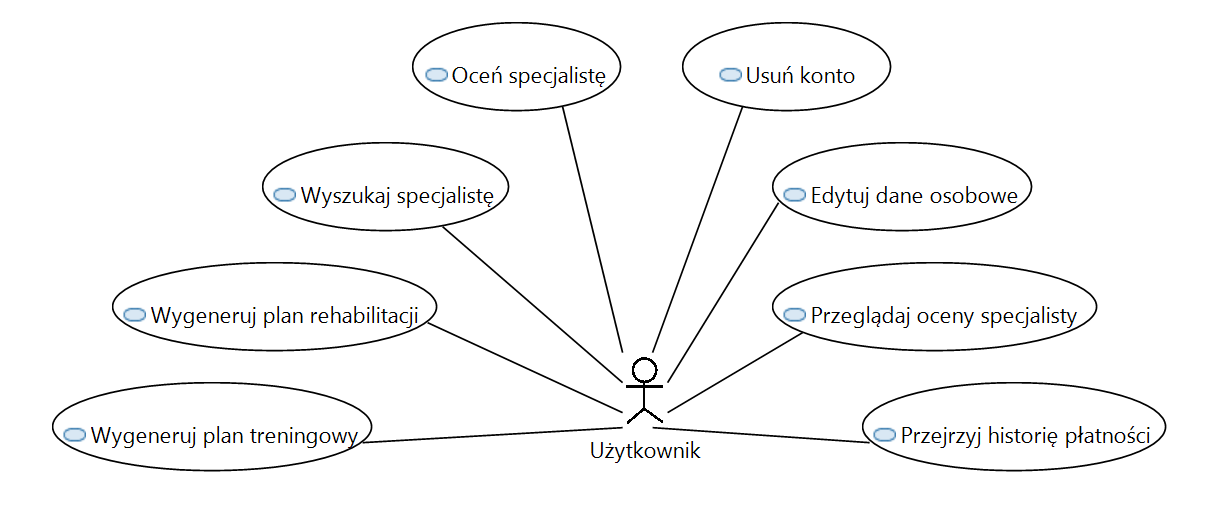
\includegraphics{diagrams/use_cases/uzytkownik.png}}

{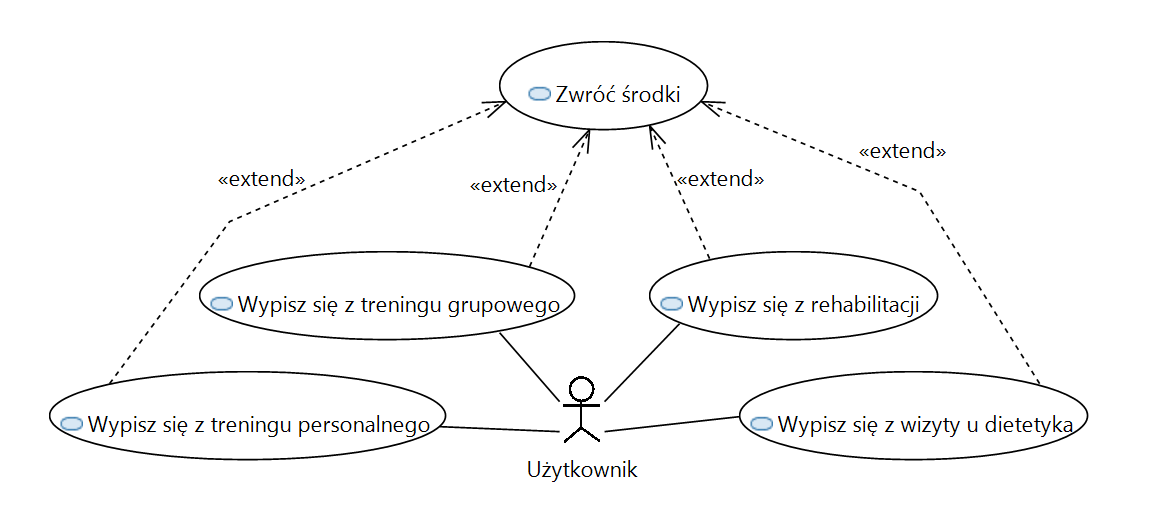
\includegraphics{diagrams/use_cases/wypisywanie.png}}

{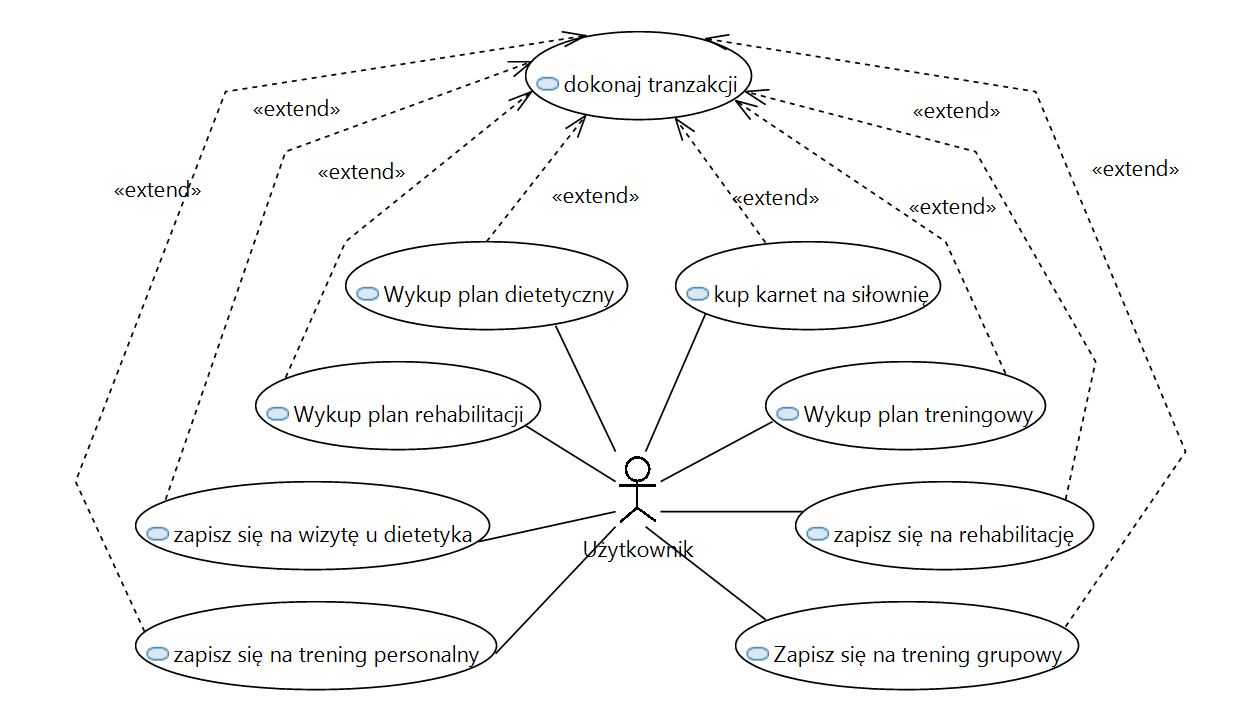
\includegraphics{diagrams/use_cases/zapisy.png}}

{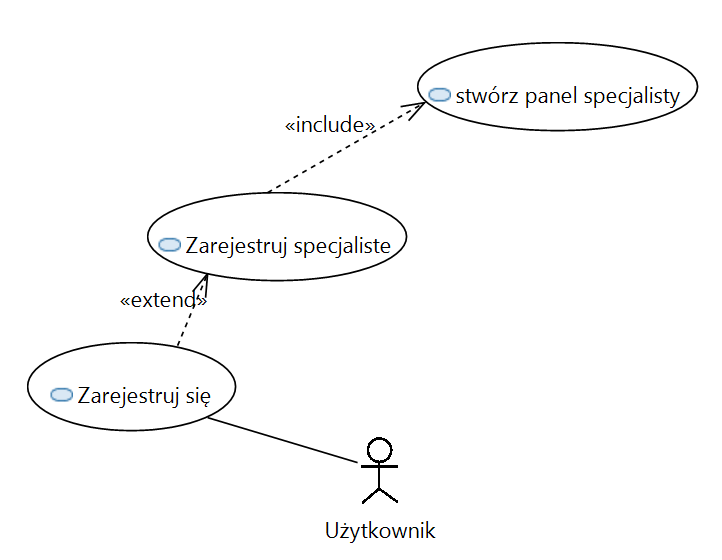
\includegraphics{diagrams/use_cases/rejestracja.png}}

\begin{enumerate}
\setcounter{enumi}{30}
\tightlist
\item
  {Zaloguj się}
\end{enumerate}

{Aktorzy biorący udział: Użytkownik.}

{Cel przypadku: Umożliwienie użytkownikowi dostępu do systemu za pomocą
autoryzacji poprzez login i hasło.}

{Warunki początkowe: Użytkownik posiada poprawny login i hasło, które
zostały już utworzone. System wymaga, aby użytkownik był uwierzytelniony
przed dostępem do chronionych zasobów.}

{Warunki końcowe: Po zalogowaniu użytkownik uzyskuje dostęp do
chronionych zasobów, które zostały mu przydzielone przez system.}

{Główny ciąg zdarzeń:}

\begin{enumerate}
\tightlist
\item
  {~Użytkownik otwiera stronę logowania.}
\item
  {System wyświetla formularz logowania z polami loginu i hasła.}
\item
  {Użytkownik wprowadza swoje dane uwierzytelniające.}
\item
  {System sprawdza poprawność wprowadzonych danych uwierzytelniających.}
\item
  {System autoryzuje użytkownika i umożliwia mu dostęp do chronionych
  zasobów.}
\end{enumerate}

{~~~~~~~~Alternatywny ciąg zdarzeń:}

\begin{itemize}
\tightlist
\item
  {Jeśli wprowadzone dane uwierzytelniające są nieprawidłowe, system
  wyświetla komunikat o błędnych danych uwierzytelniających i prosi
  użytkownika o ponowne wprowadzenie poprawnych danych. Wyświetla także
  komunikat o możliwości odzyskania hasła.\\
  \strut \\
  }
\end{itemize}

\begin{enumerate}
\setcounter{enumi}{31}
\tightlist
\item
  {Zarejestruj się}
\end{enumerate}

{Aktorzy biorący udział: Użytkownik.}

{Cel przypadku: ~Umożliwienie użytkownikowi utworzenia nowego konta w
systemie.}

{Warunki początkowe: Użytkownik nie ma jeszcze konta w systemie i chce
się zarejestrować.\\
Warunki końcowe: Po rejestracji użytkownik uzyskuje dostęp do systemu i
może korzystać z jego funkcjonalności.}

{Główny ciąg zdarzeń:}

\begin{enumerate}
\tightlist
\item
  {Użytkownik otwiera stronę rejestracji.}
\item
  {System wyświetla formularz rejestracyjny z polami do wprowadzenia
  danych użytkownika.}
\item
  {Użytkownik wprowadza swoje dane osobowe i dane do logowania (login i
  hasło).}
\item
  {System sprawdza poprawność wprowadzonych danych i wyświetla komunikat
  o sukcesie rejestracji.}
\item
  {Użytkownik zostaje automatycznie zalogowany do systemu i uzyskuje
  dostęp do funkcjonalności systemu.}
\end{enumerate}

{~~~~~~~~Alternatywny ciąg zdarzeń:}

\begin{itemize}
\tightlist
\item
  {Jeśli wprowadzone dane są niepoprawne, system wyświetla komunikat o
  błędzie i prosi użytkownika o poprawienie danych.}
\item
  {Jeśli login wprowadzony przez użytkownika jest już zajęty, system
  wyświetla komunikat o błędzie i prosi użytkownika o wybór innego
  loginu.}
\item
  {Użytkownik otrzymuje wiadomość e-mail z prośbą o potwierdzenie
  rejestracji klikając w link aktywacyjny, który weryfikuje poprawność
  wprowadzonych danych.}
\item
  {Jeśli użytkownik nie potwierdzi rejestracji w określonym czasie,
  system usuwa konto użytkownika i informuje go o tym.\\
  }
\end{itemize}

{}

\begin{enumerate}
\setcounter{enumi}{32}
\tightlist
\item
  {Zarejestruj specjalistę}
\end{enumerate}

{Aktorzy biorący udział: Użytkownik.}

{Cel przypadku: ~Umożliwienie użytkownikowi utworzenia nowego konta w
systemie jako specjalista.}

{Warunki początkowe: Użytkownik nie ma jeszcze konta jako specjalista w
systemie i chce się zarejestrować.\\
Warunki końcowe: Po rejestracji użytkownik uzyskuje dostęp do systemu i
może korzystać z jego rozszerzonych funkcjonalności jako specjalista.}

{Główny ciąg zdarzeń:}

\begin{enumerate}
\tightlist
\item
  {Użytkownik otwiera stronę rejestracji.}
\item
  {System wyświetla formularz rejestracyjny z polami do wprowadzenia
  danych użytkownika i dodatkowymi danymi dotyczącymi specjalizacji.}
\item
  {Użytkownik wprowadza swoje dane osobowe i dane do logowania (login i
  hasło) oraz dane potwierdzające jego specjalizacje.}
\item
  {System sprawdza poprawność wprowadzonych danych i wyświetla komunikat
  o sukcesie rejestracji.}
\item
  {Użytkownik zostaje automatycznie zalogowany do systemu jako
  specjalista i uzyskuje dostęp do rozszerzonych funkcjonalności
  systemu.}
\end{enumerate}

{~~~~~~~~Alternatywny ciąg zdarzeń:}

\begin{itemize}
\tightlist
\item
  {Jeśli wprowadzone dane są niepoprawne, system wyświetla komunikat o
  błędzie i prosi użytkownika o poprawienie danych.}
\item
  {Jeśli login wprowadzony przez użytkownika jest już zajęty, system
  wyświetla komunikat o błędzie i prosi użytkownika o wybór innego
  loginu.}
\item
  {Użytkownik otrzymuje wiadomość e-mail z prośbą o potwierdzenie
  rejestracji klikając w link aktywacyjny, który weryfikuje poprawność
  wprowadzonych danych.}
\item
  {Jeśli użytkownik nie potwierdzi rejestracji w określonym czasie,
  system usuwa konto użytkownika i informuje go o tym.\\
  \strut \\
  }
\end{itemize}

\begin{enumerate}
\setcounter{enumi}{33}
\tightlist
\item
  {Stwórz panel specjalisty
  \textless\textless extend\textgreater\textgreater{}}
\end{enumerate}

{Aktorzy biorący udział: Użytkownik.}

{Cel przypadku: ~Umożliwienie użytkownikowi utworzenia panelu
specjalisty, który umożliwi mu zarządzanie zasobami i danymi w systemie
dostarczając dodatkowych funkcjonalności.}

{Warunki początkowe: Użytkownik posiada konto w systemie i jest
zalogowany. System umożliwia tworzenie panelu dla specjalisty.\\
Warunki końcowe: Po stworzeniu panelu specjalista użytkownik uzyskuje
dostęp do zasobów i danych, które umożliwią mu pracę jako specjalista.}

{Główny ciąg zdarzeń:}

\begin{enumerate}
\tightlist
\item
  {Użytkownik loguje się do systemu i otwiera stronę tworzenia panelu
  specjalisty.}
\item
  {System wyświetla formularz tworzenia panelu, w którym użytkownik
  wprowadza dane potwierdzające specjalizację.}
\item
  {System tworzy nowy panel i przypisuje go do konta użytkownika jako
  panel specjalisty.}
\item
  {Użytkownik zostaje poinformowany o utworzeniu nowego panelu i
  uzyskuje dostęp do zasobów i danych, które umożliwią mu zarządzanie
  swoją pracą w systemie jako specjalista.}
\end{enumerate}

{~~~~~~~~Alternatywny ciąg zdarzeń:}

\begin{itemize}
\tightlist
\item
  {Jeśli system napotka problem podczas tworzenia panelu, wyświetla
  komunikat o błędzie i informuje użytkownika o tym. Użytkownik może
  spróbować stworzyć panel ponownie lub skontaktować się z działem
  obsługi technicznej w celu rozwiązania problemu.\\
  \strut \\
  }
\end{itemize}

\begin{enumerate}
\setcounter{enumi}{34}
\tightlist
\item
  {Wykup plan rehabilitacji
  \textless\textless include\textgreater\textgreater{}}
\end{enumerate}

{Aktorzy biorący udział: Użytkownik.}

{Cel przypadku: ~Umożliwienie użytkownikowi dokonania płatności i
uzyskania dostępu do specjalistycznych programów rehabilitacyjnych w
systemie.}

{Warunki początkowe: Użytkownik posiada konto w systemie i jest
zalogowany. System umożliwia wykupienie planu rehabilitacji.\\
Warunki końcowe: Użytkownik dokonuje płatności i uzyskuje dostęp do
specjalistycznych programów rehabilitacyjnych w systemie.}

{Główny ciąg zdarzeń:}

\begin{enumerate}
\tightlist
\item
  {Użytkownik loguje się do systemu i otwiera stronę wykupu planu
  rehabilitacji.}
\item
  {System wyświetla listę dostępnych planów rehabilitacyjnych wraz z ich
  opisem i cenami.}
\item
  {Użytkownik wybiera plan rehabilitacyjny, który chce wykupić i klika
  przycisk "Kup teraz".}
\item
  {System wyświetla formularz płatności, w którym użytkownik może
  wprowadzić swoje dane oraz informacje o karcie kredytowej lub innym
  sposobie płatności.}
\item
  {Użytkownik wprowadza swoje dane oraz informacje o płatności i kliknie
  przycisk "Zapłać".}
\item
  {System przetwarza płatność i udziela użytkownikowi dostępu do planu
  rehabilitacyjnego.}
\end{enumerate}

{~~~~~~~~Alternatywny ciąg zdarzeń:}

\begin{itemize}
\tightlist
\item
  {Jeśli system wykryje błąd w informacjach o płatności lub karcie
  kredytowej, wyświetla komunikat o błędzie i prosi użytkownika o
  poprawienie informacji.}
\item
  {Jeśli płatność nie zostanie zaakceptowana, system wyświetla
  informacje o nieudanej płatności i prosi użytkownika o wybranie innego
  sposobu płatności lub skontaktowanie się z działem obsługi
  technicznej.}
\item
  {Jeśli rehabilitacja jest darmowa użytkownik jedynie wprowadza swoje
  dane.}
\end{itemize}

{\hfill\break
}

\begin{enumerate}
\setcounter{enumi}{35}
\tightlist
\item
  {Wykup plan dietetyczny}
\end{enumerate}

{Aktorzy biorący udział: Użytkownik.}

{Cel przypadku: ~Umożliwienie użytkownikowi dokonania płatności i
uzyskania dostępu do indywidualnie dopasowanych planów żywieniowych i
porad dietetycznych.}

{Warunki początkowe: Użytkownik posiada konto w systemie i jest
zalogowany. System umożliwia wykupienie planu dietetycznego.\\
Warunki końcowe: Użytkownik dokonuje płatności i uzyskuje dostęp do
indywidualnie dopasowanych planów żywieniowych i porad dietetycznych w
systemie.}

{Główny ciąg zdarzeń:}

\begin{enumerate}
\tightlist
\item
  {Użytkownik loguje się do systemu i otwiera stronę wykupu planu
  dietetycznego.}
\item
  {System wyświetla listę dostępnych planów dietetycznych wraz z ich
  opisem i cenami.}
\item
  {Użytkownik wybiera plan dietetyczny, który chce wykupić i klika
  przycisk "Kup teraz".}
\item
  {System wyświetla formularz płatności, w którym użytkownik może
  wprowadzić swoje dane oraz informacje o karcie kredytowej lub innym
  sposobie płatności.}
\item
  {Użytkownik wprowadza swoje dane oraz informacje o płatności i kliknie
  przycisk "Zapłać".}
\item
  {System przetwarza płatność i udziela użytkownikowi dostępu do
  indywidualnie dopasowanych planów żywieniowych i porad dietetycznych.}
\end{enumerate}

{~~~~~~~~Alternatywny ciąg zdarzeń:}

\begin{itemize}
\tightlist
\item
  {Jeśli system wykryje błąd w informacjach o płatności lub karcie
  kredytowej, wyświetla komunikat o błędzie i prosi użytkownika o
  poprawienie informacji.}
\item
  {Jeśli płatność nie zostanie zaakceptowana, system wyświetla
  informacje o nieudanej płatności i prosi użytkownika o wybranie innego
  sposobu płatności lub skontaktowanie się z działem obsługi
  technicznej.}
\item
  {Jeśli plan dietetyczny jest darmowy użytkownik jedynie wprowadza
  swoje dane.}
\end{itemize}

{\hfill\break
}

\begin{enumerate}
\setcounter{enumi}{36}
\tightlist
\item
  {Wykup plan treningowy}
\end{enumerate}

{Aktorzy biorący udział: Użytkownik.}

{Cel przypadku: ~Umożliwienie użytkownikowi wykupienia planu
treningowego, który zostanie dostarczony przez platformę.}

{Warunki początkowe: Użytkownik musi być zalogowany na swoim koncie.\\
Warunki końcowe: Użytkownik wykupuje plan treningowy, który jest
aktualnie dostępny. Użytkownik otrzymuje potwierdzenie zakupu i plan
treningowy dostępny w jego panelu.}

{Główny ciąg zdarzeń:}

\begin{enumerate}
\tightlist
\item
  {Użytkownik wybiera z menu opcję "Wykup plan treningowy".}
\item
  {System wyświetla listę dostępnych planów treningowych wraz z cenami i
  opisami.}
\item
  {Użytkownik wybiera plan treningowy, który chce wykupić.}
\item
  {System wyświetla podsumowanie wybranego planu treningowego oraz
  informacje dotyczące płatności.}
\item
  {Użytkownik dokonuje płatności za plan treningowy.}
\item
  {System potwierdza dokonanie płatności i udostępnia użytkownikowi
  dostęp do planu treningowego w panelu użytkownika.}
\end{enumerate}

{~~~~~~~~Alternatywny ciąg zdarzeń:}

\begin{itemize}
\tightlist
\item
  {W przypadku niepowodzenia płatności, system informuje użytkownika o
  błędzie i proponuje powtórzenie transakcji lub wybór innej metody
  płatności.}
\item
  {Jeśli plan treningowy jest darmowy użytkownik jedynie wprowadza swoje
  dane.\\
  }
\end{itemize}

{}

\begin{enumerate}
\setcounter{enumi}{37}
\tightlist
\item
  {Kup karnet na siłownię}
\end{enumerate}

{Aktorzy biorący udział: Użytkownik.}

{Cel przypadku: Umożliwienie użytkownikowi zakupu karnetu na siłownię,
który pozwoli mu na korzystanie z usług siłowni przez określony czas.}

{Warunki początkowe: Użytkownik musi być zalogowany na swoim koncie.\\
Warunki końcowe: Użytkownik wykupuje plan treningowy, który jest
dostępny w panelu użytkownika. Użytkownik otrzymuje potwierdzenie zakupu
i plan treningowy dostępny w jego panelu.}

{Główny ciąg zdarzeń:}

\begin{enumerate}
\tightlist
\item
  {Użytkownik wybiera z menu opcję "Kup karnet na siłownię".}
\item
  {System wyświetla listę dostępnych karnetów wraz z cenami i opisami.}
\item
  {Użytkownik wybiera karnet, który chce kupić.}
\item
  {System wyświetla podsumowanie wybranego karnetu oraz informacje
  dotyczące płatności.}
\item
  {Użytkownik dokonuje płatności za karnet.}
\item
  {System potwierdza dokonanie płatności i udostępnia użytkownikowi
  informacje dotyczące karnetu w panelu użytkownika.}
\end{enumerate}

{~~~~~~~~Alternatywny ciąg zdarzeń:}

\begin{itemize}
\tightlist
\item
  {W przypadku niepowodzenia płatności, system informuje użytkownika o
  błędzie i proponuje powtórzenie transakcji lub wybór innej metody
  płatności.\\
  \strut \\
  }
\end{itemize}

\begin{enumerate}
\setcounter{enumi}{38}
\tightlist
\item
  {Zapisz się na trening personalny}
\end{enumerate}

{Aktorzy biorący udział: Użytkownik.}

{Cel przypadku: umożliwienie użytkownikowi zapisu na trening personalny
z trenerem siłowni.}

{Warunki początkowe: Użytkownik musi być zalogowany na swoje konto.}

{Musi być dostępna wolna godzina treningowa z wybranym trenerem.}

{Warunki końcowe: Użytkownik zostaje zapisany na trening personalny z
wybranym trenerem. System wyświetla potwierdzenie zapisu.}

{Główny ciąg zdarzeń:}

\begin{enumerate}
\tightlist
\item
  {Użytkownik wybiera z menu opcję "Zapisz się na trening personalny".}
\item
  {System wyświetla listę dostępnych trenerów oraz wolne godziny
  treningowe.}
\item
  {Użytkownik wybiera trenera oraz godzinę treningową, na którą chce się
  zapisać.}
\item
  {System wyświetla podsumowanie wyboru oraz informacje o cenie
  treningu.}
\item
  {Użytkownik potwierdza zapis na trening personalny dokonując
  płatności.}
\item
  {System wyświetla potwierdzenie zapisu i informacje o treningu.}
\end{enumerate}

{~~~~~~~~Alternatywny ciąg zdarzeń:}

\begin{itemize}
\tightlist
\item
  {Jeśli nie ma wolnej godziny z wybranym trenerem, system informuje
  użytkownika o braku dostępności i proponuje wybór innego trenera lub
  godziny.}
\item
  {W przypadku braku potwierdzenia zapisu przez użytkownika, system
  anuluje proces zapisu na trening personalny.}
\item
  {Jeśli z pewnych przyczyn trening nie będzie mógł się odbyć użytkownik
  zostanie poproszony o wybranie nowego terminu lub otrzyma zwrot
  kosztów za zapis.}
\item
  {W przypadku, gdy trening personalny jest darmowy użytkownik jedynie
  będzie musiał wprowadzić swoje dane}
\item
  {W przypadku niepowodzenia płatności, system informuje użytkownika o
  błędzie i proponuje powtórzenie transakcji lub wybór innej metody
  płatności.\\
  \strut \\
  \strut \\
  }
\end{itemize}

\begin{enumerate}
\setcounter{enumi}{39}
\tightlist
\item
  {Zapisz się na rehabilitację}
\end{enumerate}

{Aktorzy biorący udział: Użytkownik.}

{Cel przypadku: Umożliwienie użytkownikowi zapisu na rehabilitację}

{Warunki początkowe: Użytkownik musi być zalogowany na swoje konto.
Muszą być dostępne wolne terminy na rehabilitację.}

{Warunki końcowe: Użytkownik zostaje zapisany na wybraną rehabilitację.
System wyświetla potwierdzenie zapisu.}

{Główny ciąg zdarzeń:}

\begin{enumerate}
\tightlist
\item
  {Użytkownik wybiera z menu opcję "Zapisz się na rehabilitację".}
\item
  {System wyświetla listę dostępnych rehabilitacji oraz wolne terminy.}
\item
  {Użytkownik wybiera rehabilitację na który chce się zapisać oraz jej
  termin.}
\item
  {System wyświetla podsumowanie wyboru oraz informacje o cenie
  rehabilitacji.}
\item
  {Użytkownik potwierdza zapis na rehabilitację.}
\item
  {System wyświetla potwierdzenie zapisu i informacje o rehabilitacji.}
\end{enumerate}

{~~~~~~~~Alternatywny ciąg zdarzeń:}

\begin{itemize}
\tightlist
\item
  {Jeśli nie ma wolnego terminu w wybranej placówce, system informuje
  użytkownika o braku dostępności i proponuje wybór innej placówki lub
  terminu.}
\item
  {W przypadku braku potwierdzenia zapisu przez użytkownika, system
  anuluje proces zapisu na rehabilitację.}
\item
  {W przypadku niepowodzenia płatności, system informuje użytkownika o
  błędzie i proponuje powtórzenie transakcji lub wybór innej metody
  płatności.}
\item
  {Jeśli rehabilitacja jest darmowa użytkownik zostanie poproszony
  jedynie o podanie swoich danych osobowych.}
\end{itemize}

{\hfill\break
}

\begin{enumerate}
\setcounter{enumi}{40}
\tightlist
\item
  {Zapisz się na wizytę u dietetyka}
\end{enumerate}

{Aktorzy biorący udział: Użytkownik.}

{Cel przypadku: Zapisanie się na wizytę u dietetyka w celu uzyskania
porady i pomocy w zakresie odżywiania.}

{Warunki początkowe: Użytkownik jest zalogowany w systemie.}

{W systemie istnieją wolne terminy dla dietetyka.}

{Warunki końcowe: Użytkownik zostaje zapisany na wizytę u dietetyka w
wybranym terminie. System pobiera opłatę za wizytę z konta użytkownika.}

{Główny ciąg zdarzeń:}

\begin{enumerate}
\tightlist
\item
  {Użytkownik wybiera opcję "Zapisz się na wizytę u dietetyka" w menu.}
\item
  {System wyświetla dostępne terminy u dietetyka.}
\item
  {Użytkownik wybiera dogodny dla siebie termin wizyty.}
\item
  {System wyświetla podsumowanie wizyty, w tym jej cenę.}
\item
  {Użytkownik potwierdza wizytę i opłaca ją z konta.}
\item
  {System zapisuje wizytę użytkownika i wysyła mu potwierdzenie.}
\end{enumerate}

{~~~~~~~~Alternatywny ciąg zdarzeń:}

\begin{itemize}
\tightlist
\item
  {W przypadku braku wolnych terminów system informuje użytkownika o tym
  i proponuje wybór innego terminu.}
\item
  {W przypadku braku wystarczającej ilości środków na koncie, system
  prosi użytkownika o doładowanie konta lub wybór innej formy
  płatności.}
\end{itemize}

{\hfill\break
}

\begin{enumerate}
\setcounter{enumi}{41}
\tightlist
\item
  {Zapisz się na trening grupowy}
\end{enumerate}

{Aktorzy biorący udział: Użytkownik.}

{Cel przypadku: Zapisanie się użytkownika na trening grupowy w wybranym
terminie.}

{Warunki początkowe: Użytkownik jest zalogowany do swojego konta.
Użytkownik ma dostęp do kalendarza treningów grupowych. W systemie
istnieją dostępne treningi grupowe z wolnymi miejscami.}

{Warunki końcowe: Użytkownik zostaje zapisany na wybrany przez siebie
trening grupowy. W systemie odnotowana jest informacja o zapisie
użytkownika na trening.}

{Główny ciąg zdarzeń:}

\begin{enumerate}
\tightlist
\item
  {Użytkownik wybiera opcję "Zapisz się na trening grupowy".}
\item
  {System wyświetla kalendarz z dostępnymi terminami treningów
  grupowych.}
\item
  {Użytkownik wybiera wybrany termin treningu.}
\item
  {System wyświetla szczegóły treningu (np. nazwa, prowadzący, czas
  trwania).}
\item
  {Użytkownik potwierdza wybór treningu dokonując płatności za trening.}
\item
  {System zapisuje użytkownika na trening grupowy.}
\end{enumerate}

{~~~~~~~~Alternatywny ciąg zdarzeń:}

\begin{itemize}
\tightlist
\item
  {Jeśli w wybranym terminie nie ma wolnych miejsc na treningu grupowym,
  system wyświetla informację o braku miejsc i proponuje wybór innego
  terminu.}
\item
  {Użytkownik ma możliwość anulowania zapisu na trening grupowy przed
  rozpoczęciem treningu. W takim przypadku system usuwa informację o
  zapisie użytkownika na trening. W przypadku anulowania zapisu
  przynajmniej tydzień przed rozpoczęciem treningu środki na konto za
  trening zostają zwrócone na konto użytkownika.}
\item
  {W przypadku braku wystarczającej ilości środków na koncie, system
  prosi użytkownika o doładowanie konta lub wybór innej formy
  płatności.}
\item
  {Jeśli trening grupowy jest darmowy użytkownik jest proszony jedynie o
  wprowadzenie swoich danych osobowych.\\
  }
\end{itemize}

{}

\begin{enumerate}
\setcounter{enumi}{42}
\tightlist
\item
  {Wypisz się z treningu personalnego}
\end{enumerate}

{Aktorzy biorący udział: Użytkownik.}

{Cel przypadku: Wypisanie się użytkownika z treningu personalnego.}

{Warunki początkowe: Użytkownik musi być zalogowany i zapisany na
trening personalny. }

{Warunki końcowe: Trening zostaje odwołany. Trener personalny dostaje
informację poprzez aplikację. Jeśli trening został opłacony zostają
zwrócone środki lub ich część.}

{Główny ciąg zdarzeń: }

\begin{enumerate}
\tightlist
\item
  {Użytkownik wchodzi w panel nadchodzących spotkań.}
\item
  {Użytkownik wybiera interesujący go trening.}
\item
  {Użytkownik klika przycisk ``usuń''.}
\end{enumerate}

{~~~~~~~~Alternatywny ciąg zdarzeń:}

\begin{itemize}
\tightlist
\item
  {Jeśli trening z innych przyczyn nie jest już dostępny użytkownik
  dostaję informację, że dany trening jest już usunięty.}
\item
  {W przypadku błędu ze strony pośrednika płatności użytkownik zostaje o
  nim poinformowany. Użytkownik może następnie ponowić zwrot środków.}
\item
  {Jeśli trening został opłacony z zaliczką, zaliczka nie jest
  zwracana.}
\end{itemize}

{}

\begin{enumerate}
\setcounter{enumi}{43}
\tightlist
\item
  {Wypisz się z rehabilitacji}
\end{enumerate}

{Aktorzy biorący udział: Użytkownik.}

{Cel przypadku: Wypisanie się użytkownika z sesji rehabilitacyjnej.}

{Warunki początkowe: Użytkownik musi być zalogowany i zapisany na sesję
rehabilitacyjną. }

{Warunki końcowe: Sesja rehabilitacyjna zostaje odwołana. Fizjoterapeuta
dostaje informację poprzez aplikację. Jeśli sesja rehabilitacyjna
została opłacona zostają zwrócone środki lub ich część.}

{Główny ciąg zdarzeń: }

\begin{enumerate}
\tightlist
\item
  {Użytkownik wchodzi w panel nadchodzących spotkań.}
\item
  {Użytkownik wybiera interesującą go sesję.}
\item
  {Użytkownik klika przycisk ``usuń''.}
\end{enumerate}

{~~~~~~~~Alternatywny ciąg zdarzeń:}

\begin{itemize}
\tightlist
\item
  {Jeśli sesja z innych przyczyn nie jest już dostępna użytkownik
  dostaję informację, że dana sesja jest już usunięta.}
\item
  {W przypadku błędu ze strony pośrednika płatności użytkownik zostaje o
  nim poinformowany. Użytkownik może następnie ponowić zwrot środków.}
\item
  {Jeśli sesja została opłacona z zaliczką, zaliczka nie jest zwracana.}
\end{itemize}

{}

\begin{enumerate}
\setcounter{enumi}{44}
\tightlist
\item
  {Wypisz się z wizyty u dietetyka}
\end{enumerate}

{Aktorzy biorący udział: Użytkownik.}

{Cel przypadku: Wypisanie się użytkownika z wizyty.}

{Warunki początkowe: Użytkownik musi być zalogowany i zapisany na
wizytę. }

{Warunki końcowe: Wizyta zostaje odwołana. Dietetyk dostaje informację
poprzez aplikację. Jeśli wizyta została opłacona zostają zwrócone środki
lub ich część.}

{Główny ciąg zdarzeń: }

\begin{enumerate}
\tightlist
\item
  {Użytkownik wchodzi w panel nadchodzących spotkań.}
\item
  {Użytkownik wybiera interesującą go wizytę.}
\item
  {Użytkownik klika przycisk ``usuń''.}
\end{enumerate}

{~~~~~~~~Alternatywny ciąg zdarzeń:}

\begin{itemize}
\tightlist
\item
  {Jeśli wizyta z innych przyczyn nie jest już dostępna użytkownik
  dostaję informację, że dana wizyta jest już usunięta.}
\item
  {W przypadku błędu ze strony pośrednika płatności użytkownik zostaje o
  nim poinformowany. Użytkownik może następnie ponowić zwrot środków.}
\item
  {Jeśli sesja została opłacona z zaliczką, zaliczka nie jest zwracana.}
\end{itemize}

{}

\begin{enumerate}
\setcounter{enumi}{45}
\tightlist
\item
  {Wypisz się z treningu grupowego}
\end{enumerate}

{Aktorzy biorący udział: Użytkownik.}

{Cel przypadku: Wypisanie się użytkownika z treningu grupowego.}

{Warunki początkowe: Użytkownik musi być zalogowany i zapisany na
trening grupowy. }

{Warunki końcowe: Użytkownik jest wypisany z treningu. Jeśli trening
został opłacony zostają zwrócone środki lub ich część.}

{Główny ciąg zdarzeń: }

\begin{enumerate}
\tightlist
\item
  {Użytkownik wchodzi w panel nadchodzących spotkań.}
\item
  {Użytkownik wybiera interesujący go trening.}
\item
  {Użytkownik klika przycisk ``usuń''.}
\end{enumerate}

{~~~~~~~~Alternatywny ciąg zdarzeń:}

\begin{itemize}
\tightlist
\item
  {Jeśli trening z innych przyczyn nie jest już dostępny użytkownik
  dostaję informację, że dany trening jest już usunięty.}
\item
  {W przypadku błędu ze strony pośrednika płatności użytkownik zostaje o
  nim poinformowany. Użytkownik może następnie ponowić zwrot środków.}
\item
  {Jeśli trening został opłacony z zaliczką, zaliczka nie jest
  zwracana.}
\end{itemize}

{}

\begin{enumerate}
\setcounter{enumi}{46}
\tightlist
\item
  {Wygeneruj plan treningowy}
\end{enumerate}

{Aktorzy biorący udział: Użytkownik.}

{Cel przypadku: Użytkownik dostaje gotowy plan treningu wygenerowany
przez system.}

{Warunki początkowe: -}

{Warunki końcowe: Użytkownik ma zapisany plan treningowy, który został
wygenerowany.}

{Główny ciąg zdarzeń:}

\begin{enumerate}
\tightlist
\item
  {Użytkownik wchodzi w sekcję ``moje plany''.}
\item
  {Użytkownik klika przycisk ``wygeneruj plan''.}
\item
  {Użytkownik podaje potrzebne informacje w formularzu.}
\item
  {Użytkownik dostaje gotowy plan do swojej sekcji ``moje plany''.}
\end{enumerate}

{}

\begin{enumerate}
\setcounter{enumi}{47}
\tightlist
\item
  {Wygeneruj plan rehabilitacji}
\end{enumerate}

{Aktorzy biorący udział: Użytkownik.}

{Cel przypadku: Użytkownik dostaje gotowy plan rehabilitacji
wygenerowany przez system.}

{Warunki początkowe: -}

{Warunki końcowe: Użytkownik ma zapisany plan rehabilitacji, który
został wygenerowany.}

{Główny ciąg zdarzeń:}

\begin{enumerate}
\tightlist
\item
  {Użytkownik wchodzi w sekcję ``moje plany''.}
\item
  {Użytkownik klika przycisk ``wygeneruj plan''.}
\item
  {Użytkownik podaje potrzebne informacje w formularzu.}
\item
  {Użytkownik dostaje gotowy plan do swojej sekcji ``moje plany''.}
\end{enumerate}

{}

\begin{enumerate}
\setcounter{enumi}{48}
\tightlist
\item
  {Wyszukaj specjalistę}
\end{enumerate}

{Aktorzy biorący udział: Użytkownik.}

{Cel przypadku: Wyświetlenie użytkownikowi dostępnych specjalistów.}

{Warunki początkowe: -}

{Warunki końcowe: Użytkownik widzi listę dostępnych specjalistów.}

{Główny ciąg zdarzeń:}

\begin{enumerate}
\tightlist
\item
  {Użytkownik wchodzi w sekcję ``specjaliści''.}
\item
  {Użytkownik wyszukuję dany typ specjalisty.}
\item
  {Użytkownik widzi rezultat wyszukiwania.}
\end{enumerate}

{}

\begin{enumerate}
\setcounter{enumi}{49}
\tightlist
\item
  {Oceń specjalistę}
\end{enumerate}

{Aktorzy biorący udział: Użytkownik.}

{Cel przypadku: Użytkownik wystawia subiektywną ocenę dla danego
specjalisty.}

{Warunki początkowe: Użytkownik jest zalogowany.}

{Warunki końcowe: Ocena użytkownika zostaje dodana.}

{Główny ciąg zdarzeń:}

\begin{enumerate}
\tightlist
\item
  {Użytkownik wchodzi w sekcję ``specjaliści''.}
\item
  {Użytkownik wyszukuję konkretnego specjalistę.}
\item
  {Użytkownik wystawia ocenę i opis swoich odczuć co do obsługi.}
\end{enumerate}

{}

\begin{enumerate}
\setcounter{enumi}{50}
\tightlist
\item
  {Przeglądaj oceny specjalisty}
\end{enumerate}

{Aktorzy biorący udział: Użytkownik.}

{Cel przypadku: Wyświetlenie użytkownikowi ocen dla danego specjalisty.}

{Warunki początkowe: -}

{Warunki końcowe: Użytkownik widzi oceny dla danego specjalisty..}

{Główny ciąg zdarzeń:}

\begin{enumerate}
\tightlist
\item
  {Użytkownik wchodzi w sekcję ``specjaliści''.}
\item
  {Użytkownik wyszukuję konkretnego specjalistę.}
\item
  {Użytkownik widzi rezultat wyszukiwania: imię, nazwisko, stanowisko,
  dostępne lokacje, średnią ocen w skali 1-5 i poszczególne oceny..}
\end{enumerate}

{}

\begin{enumerate}
\setcounter{enumi}{51}
\tightlist
\item
  {Edytuj dane osobowe}
\end{enumerate}

{Aktorzy biorący udział: Użytkownik.}

{Cel przypadku: Zmiana danych osobowych użytkownika.}

{Warunki początkowe: Użytkownik jest zalogowany.}

{Warunki końcowe: Użytkownik ma zmienione dane w systemie.}

{Główny ciąg zdarzeń:}

\begin{enumerate}
\tightlist
\item
  {Użytkownik wchodzi w sekcję ``ja''.}
\item
  {Użytkownik zmienia dane w polach, które go interesują.}
\item
  {Użytkownik klika ``potwierdź''.}
\end{enumerate}

{}

\begin{enumerate}
\setcounter{enumi}{52}
\tightlist
\item
  {Przejrzyj historię płatności}
\end{enumerate}

{Aktorzy biorący udział: Użytkownik.}

{Cel przypadku: Przejrzenie historii płatności użytkownika}

{Warunki początkowe: Użytkownik jest zalogowany.}

{Warunki końcowe: Użytkownik widzi swoją historię płatności.}

{Główny ciąg zdarzeń:}

\begin{enumerate}
\tightlist
\item
  {Użytkownik wchodzi w sekcję ``ja''.}
\item
  {System wyświetla szczegółową historię płatności użytkownika, w tym
  daty, kwoty oraz rodzaj płatności.}
\item
  {Użytkownik może przeglądać historię płatności, a także eksportować ją
  do pliku CSV lub PDF.}
\end{enumerate}

{}

\begin{enumerate}
\setcounter{enumi}{53}
\tightlist
\item
  {Usuń konto}
\end{enumerate}

{Aktorzy biorący udział: Użytkownik.}

{Cel przypadku: Usunięcie konta użytkownika.}

{Warunki początkowe: Użytkownik jest zalogowany.}

{Warunki końcowe: Konto użytkownika zostaje usunięte, lecz informacje o
płatnościach i karnetach zostają zachowane.}

{Główny ciąg zdarzeń:}

\begin{enumerate}
\tightlist
\item
  {Użytkownik wchodzi w sekcję ``ja''.}
\item
  {Użytkownik klika ``usuń konto''.}
\item
  {Użytkownik klika ``potwierdź''.}
\end{enumerate}

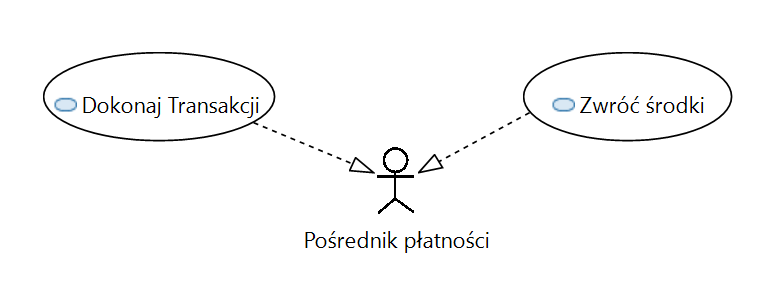
\includegraphics{diagrams/use_cases/posrednik_platnosci.png}

\hypertarget{h.q7tyc5bsqba0}{%
\subsection{\texorpdfstring{{Panel zarządzania sklepem
stacjonarnym:}}{Panel zarządzania sklepem stacjonarnym:}}\label{h.q7tyc5bsqba0}}
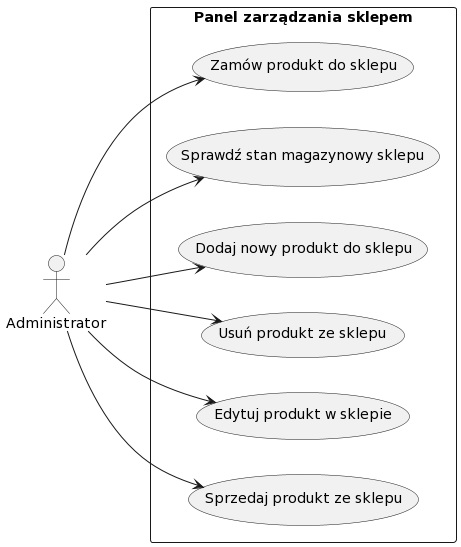
\includegraphics{diagrams/use_cases/sklep.png}
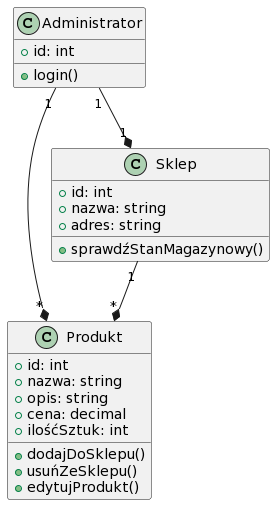
\includegraphics{diagrams/class/sklep_klasy.png}
\begin{enumerate}
\setcounter{enumi}{54}
\tightlist
\item
  {Zamów produkt do sklepu}
\end{enumerate}

{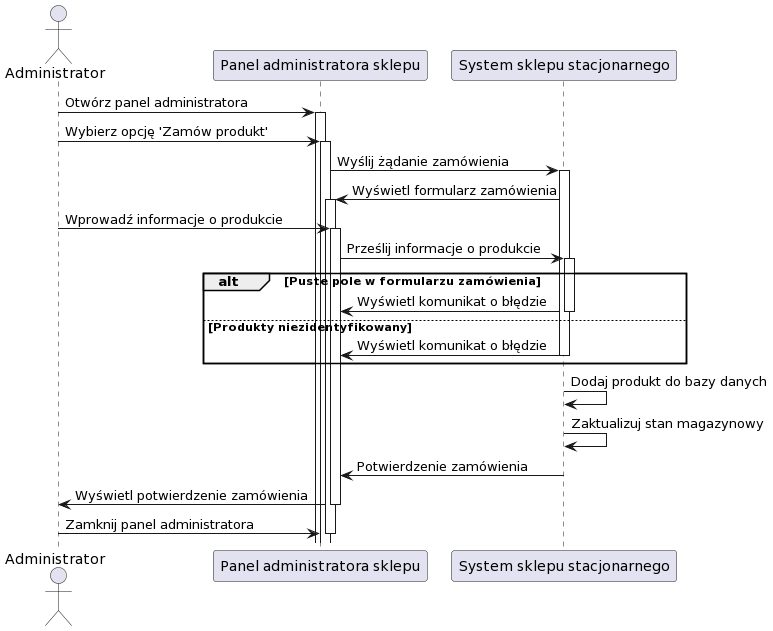
\includegraphics{diagrams/sequence/sklep_zamow_produkt_do_sklepu.png}}

\item
{Aktorzy biorący udział: Administrator}

{Cel przypadku: Zamówienie produktu do sklepu stacjonarnego}

{Warunki początkowe: Administrator jest zalogowany do panelu
administratora sklepu stacjonarnego i posiada uprawnienia do dodawania
produktów.}

{Warunki końcowe: Nowy produkt zostaje dodany do bazy danych sklepu
stacjonarnego, liczba sztuk w magazynie zostaje zaktualizowana.}

{Główny ciąg zdarzeń:}

\begin{enumerate}
\tightlist
\item
  {Administrator otwiera panel administratora sklepu stacjonarnego.}
\item
  {Administrator wybiera opcję "Zamów produkt".}
\item
  {System wyświetla formularz zamówienia, który wymaga podania
  informacji o produkcie, takie jak nazwa, opis, cena i ilość.}
\item
  {Administrator wprowadza informacje o nowym produkcie i klika przycisk
  "Zamów".}
\item
  {System dodaje produkt do bazy danych sklepu stacjonarnego.}
\end{enumerate}

{Alternatywne ciągi zdarzeń:}

{4a. Administrator zostawia puste pole wymagane w formularzu
zamówienia.}

\begin{itemize}
\tightlist
\item
  {System wyświetla komunikat o błędzie i wymaga uzupełnienia pól
  wymaganych.}
\end{itemize}

{4b. Administrator wprowadza informacje o produkcie, którego nie ma w
bazie danych sklepu stacjonarnego.}

\begin{itemize}
\tightlist
\item
  {System wyświetla komunikat o błędzie i wymaga wprowadzenia innych
  informacji lub edycji istniejącego produktu.}
\end{itemize}

{}

\begin{enumerate}
\setcounter{enumi}{55}
\tightlist
\item
  {Sprawdź stan magazynowy sklepu}
\end{enumerate}

{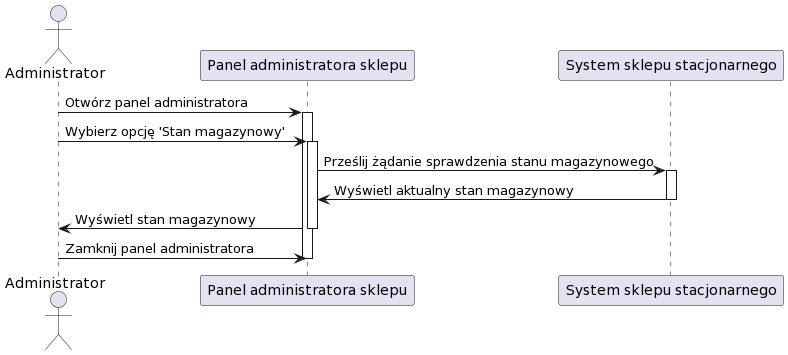
\includegraphics{diagrams/sequence/sklep_sprawdz_stan_magazynowy.png}}

{Aktorzy biorący udział: Administrator}

{Cel przypadku: Sprawdzenie stanu magazynowego sklepu stacjonarnego}

{Warunki początkowe: Administrator jest zalogowany do panelu
administratora sklepu stacjonarnego i posiada uprawnienia do sprawdzania
stanu magazynowego.}

{Warunki końcowe: Administrator widzi aktualny stan magazynowy sklepu
stacjonarnego.}

{Główny ciąg zdarzeń:}

\begin{enumerate}
\tightlist
\item
  {Administrator otwiera panel administratora sklepu stacjonarnego.}
\item
  {Administrator wybiera opcję "Stan magazynowy".}
\item
  {System wyświetla aktualny stan magazynowy sklepu stacjonarnego.}
\end{enumerate}

{Alternatywne ciągi zdarzeń:}

{Brak alternatywnych ciągów zdarzeń.}

{}

\begin{enumerate}
\setcounter{enumi}{56}
\tightlist
\item
  {Dodaj nowy produkt do sklepu}
\end{enumerate}

{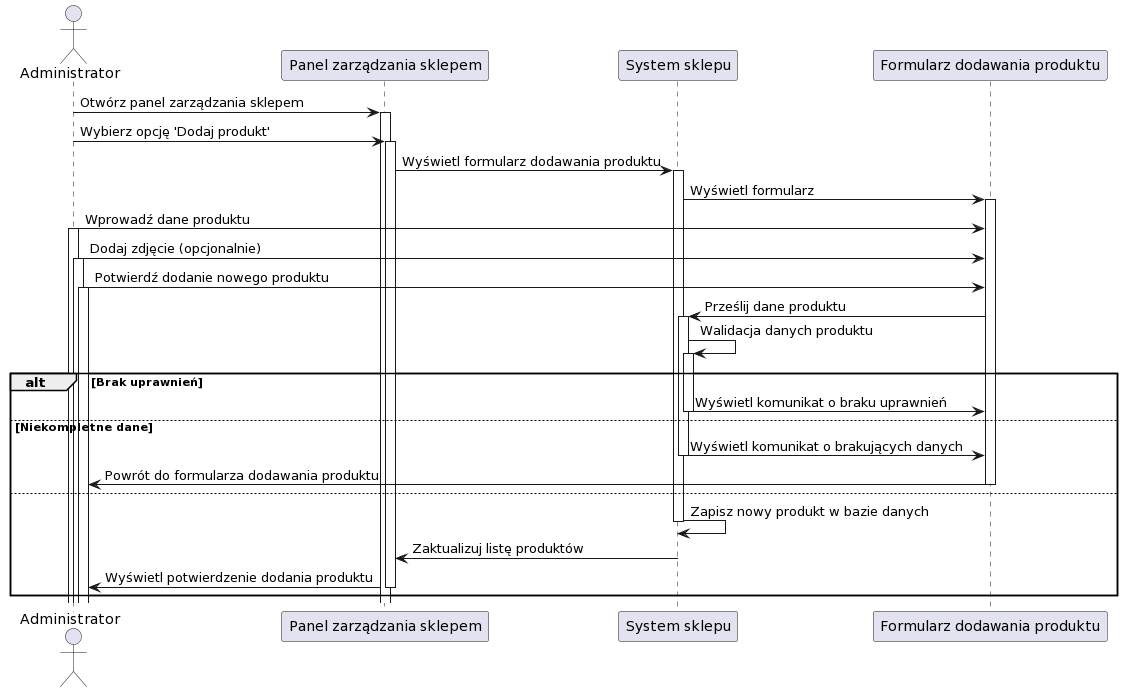
\includegraphics{diagrams/sequence/sklep_dodaj_nowy_produkt.png}}

{Aktorzy biorący udział: Administrator}

{Cel przypadku: Dodanie nowego produktu do sklepu}

{Warunki początkowe: Administrator jest zalogowany do systemu i posiada
uprawnienia do dodawania nowych produktów.}

{Warunki końcowe: Nowy produkt zostaje dodany do sklepu i jest dostępny
dla klientów.}

{Główny ciąg zdarzeń:}

\begin{enumerate}
\tightlist
\item
  {Administrator otwiera panel zarządzania sklepem.}
\item
  {Administrator wybiera opcję "Dodaj produkt".}
\item
  {System wyświetla formularz dodawania produktu.}
\item
  {Administrator wprowadza nazwę, opis, cenę oraz ilość dostępnych sztuk
  nowego produktu.}
\item
  {Administrator dodaje zdjęcie produktu, jeśli jest to wymagane.}
\item
  {Administrator potwierdza dodanie nowego produktu do sklepu.}
\item
  {System zapisuje nowy produkt w bazie danych.}
\item
  {Nowy produkt jest widoczny w sklepie dla klientów.}
\end{enumerate}

{Alternatywne ciągi zdarzeń:}

\begin{itemize}
\tightlist
\item
  {W przypadku braku uprawnień, system wyświetla odpowiedni komunikat i
  nie pozwala na dodanie nowego produktu.}
\item
  {Jeśli któryś z wymaganych pól nie zostanie wypełniony, system
  wyświetla komunikat i zwraca użytkownika do formularza dodawania
  produktu, aby wprowadził brakujące dane.}
\end{itemize}

{}

\begin{enumerate}
\setcounter{enumi}{57}
\tightlist
\item
  {Usuń produkt ze sklepu}
\end{enumerate}

{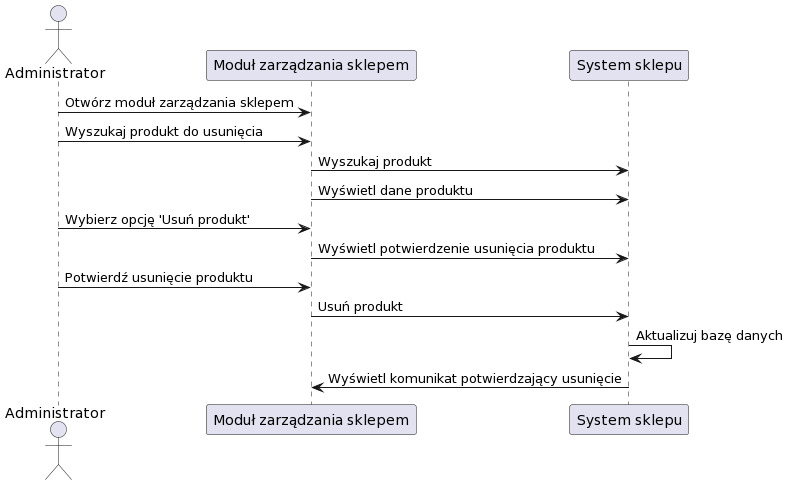
\includegraphics{diagrams/sequence/sklep_usun_produkt_ze_sklepu.png}}

{Aktorzy biorący udział: Administrator}

{Cel przypadku: Usunięcie produktu ze sklepu}

{Warunki początkowe: Administrator jest zalogowany do systemu
zarządzania siłownią i posiada uprawnienia do usuwania produktów ze
sklepu.}

{Warunki końcowe: Produkt został usunięty ze sklepu.}

{Główny ciąg zdarzeń:}

\begin{enumerate}
\tightlist
\item
  {Administrator otwiera moduł zarządzania sklepem.}
\item
  {Administrator wyszukuje produkt, który chce usunąć.}
\item
  {Administrator wybiera opcję "Usuń produkt".}
\item
  {System wyświetla potwierdzenie usunięcia produktu.}
\item
  {Administrator potwierdza usunięcie produktu.}
\item
  {System usuwa produkt ze sklepu.}
\item
  {System wyświetla komunikat potwierdzający usunięcie produktu.}
\end{enumerate}

{Alternatywne ciągi zdarzeń:}

{5a. Jeśli administrator zrezygnuje z usunięcia produktu, system anuluje
proces usuwania i wraca do poprzedniego stanu.}

{}

{}

\begin{enumerate}
\setcounter{enumi}{58}
\tightlist
\item
  {Edytuj produkt w sklepie}
\end{enumerate}

{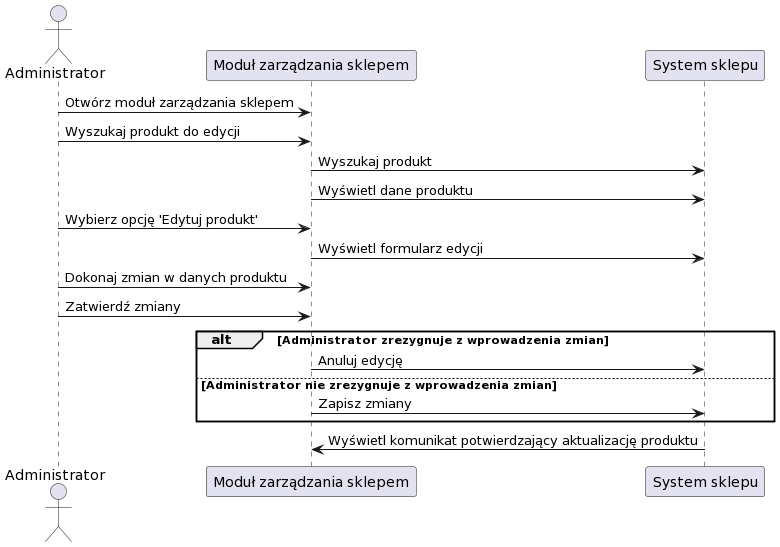
\includegraphics{diagrams/sequence/sklep_edycja_produktu.png}}

{Aktorzy biorący udział: Administrator}

{Cel przypadku: Edycja produktu w sklepie}

{Warunki początkowe: Administrator jest zalogowany do systemu
zarządzania siłownią i posiada uprawnienia do edycji produktów w
sklepie.}

{Warunki końcowe: Produkt został zaktualizowany w sklepie.}

{Główny ciąg zdarzeń:}

\begin{enumerate}
\tightlist
\item
  {Administrator otwiera moduł zarządzania sklepem.}
\item
  {Administrator wyszukuje produkt, który chce edytować.}
\item
  {Administrator wybiera opcję "Edytuj produkt".}
\item
  {System wyświetla formularz edycji produktu.}
\item
  {Administrator dokonuje zmian w danych produktu.}
\item
  {Administrator zatwierdza zmiany.}
\item
  {System zapisuje zmiany w danych produktu.}
\item
  {System wyświetla komunikat potwierdzający aktualizację produktu.}
\end{enumerate}

{Alternatywne ciągi zdarzeń:}

{5a. Jeśli administrator zrezygnuje z wprowadzenia zmian, system anuluje
proces edycji i wraca do poprzedniego stanu.}

{}

\begin{enumerate}
\setcounter{enumi}{59}
\tightlist
\item
  {Sprzedaj produkt ze sklepu}
\end{enumerate}

{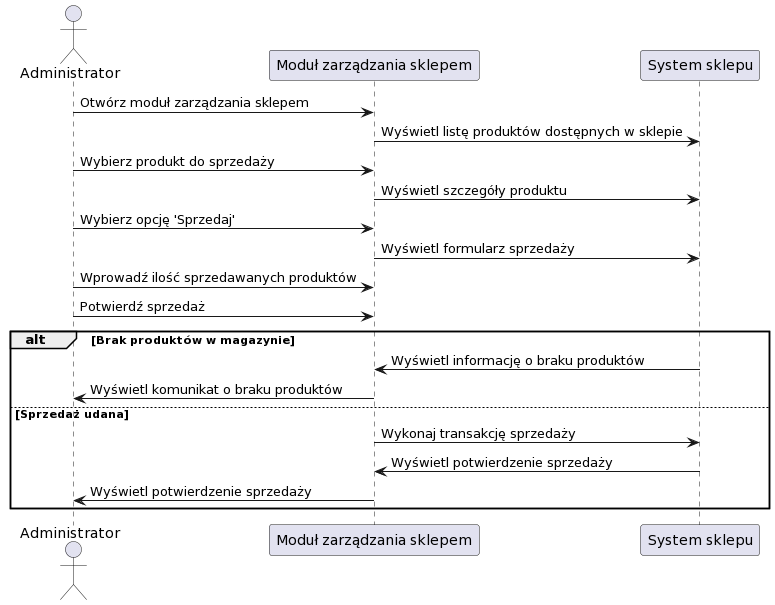
\includegraphics{diagrams/sequence/sklep_sprzedaj_produkt.png}}

{Aktorzy biorący udział: Administrator}

{Cel przypadku: Dokonanie sprzedaży produktu ze sklepu stacjonarnego}

{Warunki początkowe: Administrator jest zalogowany do systemu i posiada
uprawnienia do sprzedaży produktów ze sklepu stacjonarnego. W sklepie
znajduje się co najmniej jeden produkt do sprzedania.}

{Warunki końcowe: zaktualizowanie stanu magazynowego produktu w
systemie.}

{Główny ciąg zdarzeń:}

\begin{enumerate}
\tightlist
\item
  {Administrator otwiera moduł zarządzania sklepem.}
\item
  {System wyświetla listę produktów dostępnych w sklepie stacjonarnym.}
\item
  {Administrator wybiera produkt, który chce sprzedać.}
\item
  {System wyświetla szczegóły wybranego produktu, takie jak nazwa, opis,
  cena, stan magazynowy.}
\item
  {Administrator wybiera opcję "Sprzedaj" przy wybranym produkcie.}
\item
  {System wyświetla formularz sprzedaży, w którym Administrator
  wprowadza ilość sprzedawanych produktów}
\item
  {Administrator potwierdza sprzedaż, klikając przycisk "Sprzedaj".}
\item
  {System wykonuje transakcję sprzedaży, aktualizując stan magazynowy
  produktu oraz generując potwierdzenie sprzedaży.}
\item
  {System wyświetla potwierdzenie sprzedaży wraz z informacjami o
  sprzedanym produkcie.}
\end{enumerate}

{Alternatywne ciągi zdarzeń:}

{1. Brak produktów w magazynie}

{System wyświetla informację o braku produktów w magazynie.}

{Administrator nie może dokonać sprzedaży i zamyka formularz sprzedaży.}

\begin{center}\rule{0.5\linewidth}{0.5pt}\end{center}

{}

\hypertarget{h.3q9pme6aem79}{%
\section{\texorpdfstring{{Kontrybucja:}}{Kontrybucja:}}\label{h.3q9pme6aem79}}

{Panel trenera personalnego:}

\begin{enumerate}
\tightlist
\item
  {Stwórz plan treningowy~~~~~~~~.}
\item
  {Edytuj plan treningowy~~~~~~~~.}
\item
  {Usuń plan treningowy}
\end{enumerate}

{Panel fizjoterapeuty:}

\begin{enumerate}
\setcounter{enumi}{3}
\tightlist
\item
  {Stwórz plan rehabilitacji}
\item
  {Edytuj plan rehabilitacji}
\item
  {Usuń plan rehabilitacji}
\end{enumerate}

{Panel dietetyka:}

\begin{enumerate}
\setcounter{enumi}{6}
\tightlist
\item
  {Stwórz plan dietetyczny}
\item
  {Edytuj plan dietetyczny}
\item
  {Usuń plan dietetyczny}
\end{enumerate}

{Panel specjalisty:}

\begin{enumerate}
\setcounter{enumi}{9}
\tightlist
\item
  {Zobacz panel specjalisty}
\end{enumerate}

{Panel właściciela siłowni:}

\begin{enumerate}
\setcounter{enumi}{10}
\tightlist
\item
  {Stwórz trening grupowy}
\item
  {Edytuj trening grupowy}
\item
  {Usuń trening grupowy}
\item
  {Zbanuj użytkownika}
\item
  {Dodaj specjalistę}
\item
  {Edytuj specjalistę}
\item
  {Usuń specjalistę}
\item
  {Przypisz specjalistę do budynku}
\item
  {Usuń specjalistę z budynku}
\item
  {Wypisz użytkownika z treningu personalnego}
\item
  {Wypisz użytkownika z treningu grupowego}
\item
  {Wypisz użytkownika z rehabilitacji}
\item
  {Wypisz użytkownika z wizyty u dietetyka}
\item
  {Wygeneruj statystyki}
\end{enumerate}

{Panel Administratora:}

\begin{enumerate}
\setcounter{enumi}{24}
\tightlist
\item
  {Przejrzyj historię płatności użytkownika}
\item
  {Dodaj budynek siłowni}
\item
  {Dodaj właściciela siłowni}
\item
  {Usuń budynek siłowni}
\item
  {Usuń użytkownika}
\item
  {Usuń właściciela siłowni}
\end{enumerate}

{Strefa użytkownika:}

\begin{enumerate}
\setcounter{enumi}{30}
\tightlist
\item
  {Zaloguj się}
\item
  {Zarejestruj się}
\item
  {Zarejestruj specjalistę}
\item
  {Stwórz panel specjalisty}
\item
  {Wykup plan rehabilitacji}
\item
  {Wykup plan dietetyczny}
\item
  {Wykup plan treningowy}
\item
  {Kup karnet na siłownię}
\item
  {Zapisz się na trening personalny}
\item
  {Zapisz się na rehabilitację}
\item
  {Zapisz się na wizytę u dietetyka}
\item
  {Zapisz się na trening grupowy}
\item
  {Wypisz się z treningu personalnego}
\item
  {Wypisz się z rehabilitacji}
\item
  {Wypisz się z wizyty u dietetyka}
\item
  {Wypisz się z treningu grupowego}
\item
  {Wygeneruj plan treningowy}
\item
  {Wygeneruj plan rehabilitacji}
\item
  {Wyszukaj specjalistę}
\item
  {Oceń specjalistę}
\item
  {Przeglądaj oceny specjalisty}
\item
  {Edytuj dane osobowe}
\item
  {Przejrzyj historię płatności}
\item
  {Usuń konto}
\item
  {Dokonaj transakcji}
\item
  {Zwróć środki}
\end{enumerate}

{Panel zarządzania sklepem:}

{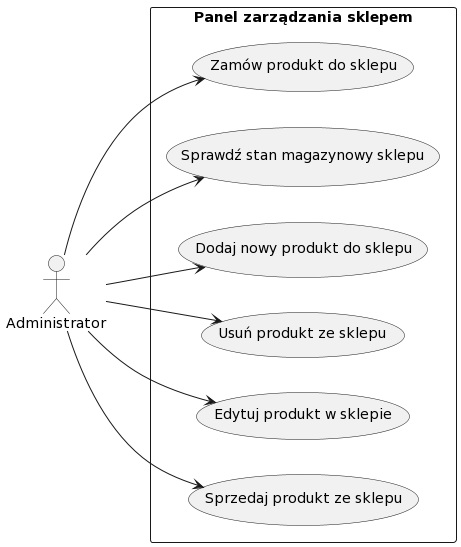
\includegraphics{diagrams/use_cases/sklep.png}}

\begin{enumerate}
\setcounter{enumi}{55}
\tightlist
\item
{Zamów produkt do sklepu}
\item
{Sprawdź stan magazynowy sklepu}
\item
{Dodaj nowy produkt do sklepu}
\item
{Usuń produkt ze sklepu}
\item
{Edytuj produkt w sklepie}
\item
{Sprzedaj produkt ze sklepu}
\end{enumerate}

{}

\end{document}
